\documentclass[a4paper,11pt]{article} % Tamaño de papel, tamaño de letra y clase LaTeX usada...

\usepackage[spanish]{babel} % Permite escribir en Castellano (tildes y ñ) e implementa...
\usepackage[utf8]{inputenc} % Permite introducir acentos y Ñ directamente.
%\usepackage[T1]{fontenc} %permite cambiar la fuente por defecto.
\usepackage{bm} % Permite letras griegas en negrita {uso: \bm{\alpha}}
\usepackage{graphicx}
\usepackage{amssymb}
\usepackage{mathtools}
\usepackage{subfigure}
\usepackage{multicol} %para añadir texto en columnas
\usepackage{float}
\usepackage{fancyhdr} %encabezados y pies de pagina
\usepackage{amsmath,amsfonts,latexsym,color,textcomp,anysize}
\usepackage[table,xcdraw]{xcolor}
\usepackage{longtable}
\usepackage{parskip}
\usepackage{hyperref}
% \usepackage{cancel} % tachar cosas \cancel{}
% \usepackage{tensor} % Notación: \tensor{T}{^a_b^c_d}
%\usepackage{mathrsfs}
\usepackage{slashed}   %\slashed{p}
\spanishdecimal{.}

\hypersetup{
    colorlinks=true,
    linkcolor=blue,
    filecolor=magenta,      
    urlcolor=cyan}


% Cuadros
\usepackage{tcolorbox}
\tcbuselibrary{listingsutf8}
\newtcolorbox{mybox}[1]
{colback=cyan!5!white,colframe=cyan!75!black,fonttitle=\bfseries,title=#1}

\newtcolorbox{mybox_green}[1]
{colback=green!5!white,colframe=green!45!black,fonttitle=\bfseries,title=#1}

\newtcolorbox{mybox_red}[1]
{colback=red!5!white,colframe=red!45!black,fonttitle=\bfseries,title=#1}


% Teoremas, lemas y demostraciones
\newtheorem{lemma}{Lemma}
\newtheorem{theorem}{Teorema}

\def\proof{\textit{Demostración: }} %\def\proof{\paragraph{Demostración: }}
\def\endproof{\hfill$\blacksquare$}


% codigo Python
\usepackage{listings}
\definecolor{dkgreen}{rgb}{0,0.6,0}
\definecolor{gray}{rgb}{0.5,0.5,0.5}
\definecolor{mauve}{rgb}{0.58,0,0.82}
\lstset{frame=tb,
  language=Python,
  aboveskip=3mm,
  belowskip=3mm,
  showstringspaces=false,
  columns=flexible,
  basicstyle={\small\ttfamily},
  numbers=none,
  numberstyle=\tiny\color{gray},
  keywordstyle=\color{blue},
  commentstyle=\color{dkgreen},
  stringstyle=\color{mauve},
  breaklines=true,
  breakatwhitespace=true,
  tabsize=3
}



%Includes "References" in the table of contents
\usepackage[nottoc]{tocbibind}
%===========================================================================================

%numerar ecuaciones con la seción
\numberwithin{equation}{section}

%===========================================================================================

\marginsize{2cm}{2cm}{1.5cm}{1.5cm} %MÁRGENES: Izq, Der, Sup, Inf.
\parindent=0mm % Sangría por defecto
\parskip=3mm % Espacio entre párrafos por defecto
%===========================================================================================
% definiciones de utilidad

%parentesis
\def\lp{\left(}
\def\rp{\right)}

\def\lc{\left[}
\def\rc{\right]}

\def\lch{\left\{}
\def\rch{\right\}}

\def\l|{\left|}
\def\r|{\right|}

\def\Lp{\Bigl(}
\def\Rp{\Bigr)}

\def\Lc{\Bigl[}
\def\Rc{\Bigr]}

\def\Lch{\Bigl\{}
\def\Rch{\Bigr\}}

%Cosas útiles

\def\Nabla{\bm \nabla}

\def\rqa{\quad \Rightarrow \quad}

\def\senc{\, \text{senc}}
%===========================================================================================
% Para poner subsubsections en letra pequeña y crear subsubsubsection en letra pequeña

\def\subsubi{\par\addtocounter{subsubsection}{1}\underline{\it\thesubsubsection.}\hskip0.5cm  \setcounter{subsubsubsection}{0}}

\newcounter{subsubsubsection}[subsubsection]
\def\subsubii{\par\addtocounter{subsubsubsection}{1}\underline{\it 
\thesubsubsection.\thesubsubsubsection.}\hskip0.5cm}
%===========================================================================================

% ================================= PORTADA =======================================

\pagestyle{empty}

\begin{document}
\renewcommand{\tablename}{Tabla}

\begin{center}

	\begin{figure}[t]
	\centering 
	
\includegraphics[width=1\linewidth]{Figuras/Fig-Logo_QS_EspanaDigital.png}
	\end{figure}

\vspace{3cm}
\rule{65mm}{0.2mm}\\
\vspace{1cm}

{\sc\LARGE El Algoritmo de Grover}

%{\sl\large Explicación del algoritmo e implementación con 2n+3 qubits }

\vspace{0.5cm}
\rule{65mm}{0.2mm}\\
\vspace{2cm}
\end{center}


\begin{tabular}{l}
{\sl\large Autor: } \\
{\bf\Large David Castaño Bandín} \\
\vspace{1em}\mbox{\hyperlink{https://www.scbi.uma.es/site/}{SCBI} (Universidad de Málaga)} \\
%
%{\sl\large Co-autores: } \\
%{\bf\large Alejandro Cano} \\
%\hyperlink{https://web.unican.es/}{UNICAN} \\
%{\bf\large Javier Sánchez} \\
%\hyperlink{https://www.cenits.es/}{Cénits} \\
%{\bf\large Alejandro Cano} \\
%\hyperlink{https://www.bsc.es/}{BSC-CNS} \\
%\vspace{1em}\mbox{} \\
%
{\sl\large Revisores:} \\
{\bf\large Javier Mas Solé} \\
Universidad de Santiago de Compostela \\
{\bf\large Andrés Gómez Tato} \\
\hyperlink{http://www.cesga.es}{CESGA}
\vspace{1em}\mbox{} \\
\end{tabular}


\begin{center}
\vspace{1cm}
{\Large 27/03/2023}
\end{center}

	\begin{figure}[b]
	\centering 
	
\includegraphics[width=1\linewidth]{Figuras/Fig-LOGOS-GOB_QS.png}
	\end{figure}

\newpage
\thispagestyle{empty}
\mbox{}

\newpage
\pagestyle{plain}
\tableofcontents
\newpage



%\textcolor{red}{Notas: }

%\textcolor{red}{- Editar la parte de la introducción donde se mencionan las secciones.}

%\textcolor{red}{- Mirar lo de usar otras transformaciones diferentes a la Hadammard (sección \ref{sub-sec_N-no-2^n})}


\newpage
\section*{Diccionario de notaciones}

\begin{table}[H]
\centering
\begin{tabular}{ll}
\hline
\textbf{$\mathcal(O)(z)$}     & Esta notación quiere decir ``del orden de $z$''.                 \\ \hline
\textbf{$N$}                  & Número de elemento del dataset en el que buscamos                \\ \hline
\textbf{$n$}                  & Número de qubits que nos hacen falta                             \\ \hline
\textbf{$M$}                  & Número de soluciones que buscamos en el dataset de $N$ elementos \\ \hline
\textbf{$t$}                  & Número de iteraciones del algoritmo de Grover                    \\ \hline
\textbf{$T$}                  & Número óptimo de iteraciones del algoritmo de Grover             \\ \hline
\textbf{$\lfloor z \rfloor $} & Redondear $z$ a un entero por truncamiento                       \\ \hline
\textbf{$\lceil z \rceil$}    & Redondear $z$ al siguiente entero.                               \\ \hline
\end{tabular}
\end{table}


\newpage
\section{Introducción}

La computación cuántica es un campo relativamente joven y en el cual hay depositadas muchas esperanzas, pues se cree que tiene el potencial de poder resolver algunos problemas con los que la computación clásica no puede lidiar. Estamos hablando de los famosos problemas de la clase de complejidad NP-hard. Sin embargo, pese a esta creencia, pocas demostraciones teóricas hay sobre el tema. La demostración más famosa es la del \textbf{Algoritmo de Shor}, que es capaz de abordar el problema de la factorización de un número en sus factores primos. Esto es porque el algoritmo es capaz de calcular los factores primos en un tiempo polinónico, frente al tiempo exponencial que requieren los mejores algoritmos clásicos. El algoritmo sobre el que tratan estas notas, el también archiconocido \textbf{Algoritmo de Grover}, no ofrece una ventaja exponencial respecto al mejor algoritmo clásico, pero si ofrece una mejora sustancial (cuadrática).

Resumiendo mucho, el algoritmo de Grover es un algoritmo de búsqueda no estructurada. El objetivo del algoritmo es encontrar un valor (o varios) en una secuencia no ordenada de $N$ componentes. Supongamos que tenemos una lista $L$ con $N$ elementos donde denominamos $L_i$, con $i=0,1,\dots,N-1$, al i-ésido elemento de la lista. Supongamos que queremos encontrar un elemento $q$ en la lista, es decir, lo que queremos encontrar es el índice $\omega$ tal que $L_\omega = q$. Si asumimos que la lista está desordenada, ningún algoritmo clásico conocido puede darnos un tiempo de búsqueda mejor que $\mathcal{O}(N)$. Es decir, el tiempo promedio de búsqueda crece linealmente con $N$, con el número de elementos entre los que buscamos. Esto es fácil de ver, pues para encontrar nuestro elemento tendremos que ir probando uno a uno los elementos de la lista. De esta forma en promedio tendremos que hacer $N/2$ pruebas para encontrar el resultado deseado. 

Este tipo de problemas se denominan problemas de \textbf{búsqueda no estructurada} o problemas de búsqueda en \textbf{conjuntos de datos (datasets) no estructurados}. Como acabamos de comentar, estos problemas requieren un tiempo polinómico (en concreto, lineal) para ser resueltos. Se engloban dentro de esta categoría también problemas que presenten un dataset con alguna clase de estructura siempre que esta no se pueda aprovechar para acelerar la búsqueda. 

La ventaja que aporta el algoritmo de Grover es \textbf{cuadrática}, ya que pasamos de necesitar un tiempo $\mathcal{O}(N)$ a un tiempo $\mathcal{O}(\sqrt{N})$. Esto puede parecer decepcionante si lo comparamos con la mejora exponencial que promete el algoritmo de Shor, pero está lejos de serlo.  Aunque a priori no parezca una mejora sustancial, cuando tratamos con valores suficientemente grandes de $N$ (datasets inmenso), la mejora en tiempo respecto a su contrapartida clásica puede ser de ordenes de magnitud, es decir, para nada despreciable. 

%El algoritmo de Grover asume un dataset no estructurado, lo cual es poco frecuente ya que se suele tener algún conocimiento sobre los datos. 
El algoritmo de Grover no hace uso de la estructura interna del dataset en el que realiza la búsqueda, lo cual lo hace genérico y aplicable a una gran variedad de casos. Los problemas de búsqueda aparecen por doquier en las ciencias computacionales, con lo que una mejora en la eficiencia de estos es de gran interés. Además, este algoritmo no solo nos sirve para búsquedas, sino que nos sirve como subrutina para conseguir un aumento de velocidad cuadrático en otros algoritmo. A esto último se lo denomina el truco de la \textbf{amplificación de la amplitud}.

En estas notas vamos a ver todo lo necesario para entender el algoritmo de Grover, hablando tanto de matemática como de implementaciones. La estructura de las notas es la siguiente. En la sección \ref{sec_geo} veremos una explicación geométrica del algoritmo, donde se usará como ejemplo el caso más simple (una solución, $N=2^n$ y distribución uniforme) y se verán las diferentes partes del algoritmo. En las siguientes secciones iremos generalizando el algoritmo a medida que relajamos las condiciones del ejemplo anterior. En la sección \ref{sec_t-sols} veremos que pasa cuando tenemos un número $M$ de soluciones (conocido $M$). En la sección \ref{sec_t_no_conocido} relajaremos la condición de conocer el número $M$ de soluciones y veremos que el algoritmo sigue siendo eficiente. Como continuación lógica de la sección anterior, en la sección \ref{sec_quantum_counting} veremos un algoritmo inspirado en el algoritmo de Shor que usa el operador de Grover para contar el número de soluciones (obtener $M$). En la sección \ref{sec_cons_imple} hablaremos sobre la implementación del difusor y como la formulación más habitual del mismo es la responsable de imponer la condición $N=2^n$. Veremos en la subseción \ref{subsec-N_neq_2n} como podemos eliminar también esta condición. Por último, en la sección \ref{sec_arbitrary_distribition} veremos que también es posible relajar la condición de partir de una distribución de probabilidad uniforme. 





% Se empieza siguiendo el paper \cite{Boyer_1998}

% Finally, we refine the argument of [1] to show that Grover’s algorithm could not be improved to require much less than half the number of table lookups that it currently makes when a 50\% probability of success is desired.

\newpage
\section{Explicación geométrica del algoritmo} \label{sec_geo}

Para facilitar la explicación y sin perdida de generalidad, pongámonos en el caso más simple de todos: queremos encontrar una única solución $| \omega_0 \rangle$ y tenemos $N=2^n$. Supongamos también que podemos partir del caso más simple, de una superposión uniforme de todos los estados. Más adelante iremos viendo generalizaciones del algoritmo para casos más complicados, como el caso de varias soluciones o el caso en el que partimos de una distribución de probabilidad aleatoria.

\subsection{Estado inicial: superposición}
			
Partimos de una superposición uniforme de $N$ estados 
\begin{equation} \label{ec_geo_phi-0_1}
| \Psi_0 \rangle = \frac{1}{\sqrt{N}}  \sum_{i=0}^{N} | i \rangle.
\end{equation}
Esto no es más que decir que al inicio de la búsqueda, todas las opciones son igualmente probables (cualquier suposición de la ubicación de la solución es tan buena como cualquier otra).


\begin{mybox}{Nota}
Recordemos que si $N=2^n$, donde $n$ es el número de qubits, este estado es fácil de construir, pues solo tenemos que aplicar puertas de Hadamard en todos los Qubits (partiendo estos del estado $|0 \rangle$):
\begin{equation} \label{ec_geo_phi_0_H}
|\Psi_0 \rangle = H^{\otimes n} |0 \rangle^{n} = \frac{1}{\sqrt{N}}  \sum_{i=0}^{N=2^n} | i \rangle.
\end{equation}
\end{mybox}

El objetivo del algoritmo de Grover es aumentar el valor del coeficiente que acompaña al estado $| \omega_0 \rangle$ que queremos encontrar, es decir, aumentar la probabilidad de que al medir, obtengamos este estado. Como la suma de todas las probabilidades tiene que ser 1, este aumento en la probabilidad del estado $| \omega_0 \rangle$ se produce a expensas de reducir la probabilidad del resto. 

	\begin{mybox}{Nota}
	Recordemos que en mecánica cuántica podemos tener un estado que sea la \textbf{superposición} 
	de varios estado (como es el caso anterior), pero al medir solo obtenemos \textbf{uno de estos 
	estado}. La probabilidad de medir cada uno de estos estados que forman la superposición es igual 
	al módulo cuadrado del coeficiente que lo acompaña en el vector de esto $| \Psi \rangle$ (el módulo 
	cuadrado de la amplitud). Este caso, vemos que todos los estados tiene probabilidad $1/N$. 
	\end{mybox}

\subsection{Amplificación de amplitud mediante iteraciones del algoritmo}

Como vamos a ver a continuación, el algoritmo de Grover tiene una interpretación geométrica muy simple: dos reflexiones que rotan el vector de estado en un plano bidimensional. 

El algoritmo de Grover consta de dos partes: un \textbf{oráculo} y un \textbf{difusor}. Para que el algoritmo maximice la probabilidad de la solución deseada tenemos realizar un número concreto de \textbf{iteraciones}. En cada iteración del algoritmo, primero se aplica el oráculo y después el difusor. Con cada iteración la probabilidad de medir la solución deseada va aumentando. Sin embargo, es muy importante aplicar el número correcto de iteraciones que nos maximiza la probabilidad, pues tanto si nos quedamos cortos como si nos pasamos, la probabilidad de medir $|\omega_0 \rangle$ disminuye. Esto se va a entender muy bien a continuación, cuando veamos la explicación geométrica. 

Pongamos el estado inicial de la Ec. (\ref{ec_geo_phi-0_1}) de una forma más adecuada para nuestro propósito
\begin{equation} \label{ec_geo_phi-0_2}
\boxed{|\Psi_0 \rangle = | \Psi (k(0),l(0)) \rangle = k(0) |\omega_0 \rangle + \sum_{i \neq \omega_0}  l(0)  |i \rangle}, \quad \text{donde} \quad \boxed{k(0) = l(0) = \frac{1}{\sqrt{N}}}.
\end{equation}
Denominaremos $k(t)$ y $l(t)$ a los coeficientes que tendremos en la t-esima iteración del algoritmo, es decir
\begin{equation} \label{ec_geo_phi-j}
\boxed{|\Psi(t) \rangle = | \Psi (k(t),l(t)) \rangle = k(t) |\omega_0 \rangle +  \sum_{i \neq \omega_0}^N l(t) |i \rangle }.
\end{equation}

Véase que aquí ya estamos adelantando que los coeficientes de todos los estados que no son el deseado son iguales en cada iteración. Nuestro vector de estado $|\Psi(t) \rangle$ vive en un espacio de Hilbert de $N$ dimensiones y los estados $| i \rangle$, con $i=0,1,\dots,N-1$ , forman una base ortogonal del espacio de Hilbert (véase que aquí se incluye $\omega_0$, pues no es nada más que un valor de $i$ concreto). Para entender bien esto, podemos fijamos en las Ecs. (\ref{ec_geo_phi-0_1}) y (\ref{ec_geo_phi-0_2}) y ver que estas no son más que la expresión de un vector como la multiplicación de unos coeficientes por los elementos de la base\footnote{Esto es en esencia lo mismo que con vectores en tres dimensiones: $\vec{r} = a \hat{x} + b \hat{y} + c \hat{z}$}. Como no podemos dibujar un vectores de más de 3 dimensiones, para explicar geométricamente el algoritmo vamos a recurrir a un truco: vamos a descomponer nuestro vector de estado en la suma de dos vectores $|\omega_0 \rangle$ y $| \omega^{\perp} \rangle$, donde este último es la suma de todos los demás elementos de la base, es decir:
\begin{equation} \label{ec_geo_phi-j-s}
\boxed{|\Psi(t) \rangle = | \Psi (k(t),l(t)) \rangle = k(t) |\omega_0 \rangle + l(t) \sqrt{N-1} | \omega^{\perp}  \rangle}, \qquad \text{donde} \qquad \boxed{| \omega^{\perp}  \rangle = \frac{1}{\sqrt{N-1}}\sum_{i \neq \omega_0}^N  |i \rangle}.
\end{equation}

	\begin{mybox}{Nota}
	Es importante darse cuenta de donde sale el factor $\sqrt{N-1}$ en la definición de 
	$|\omega^{\perp}\rangle$. Este es debido a que estamos definiendo $|\omega^{\perp}\rangle$ 
	como un vector unitario, es decir 
	\begin{equation}
	\langle \omega^{\perp}| \omega^{\perp} \rangle = 1.
	\end{equation}
	Por otro lado, $|\Psi_0\rangle$ también es unitario
	\begin{equation}
	\parallel |\Psi(t) \rangle \parallel^2 = \langle \Psi(t) | \Psi(t) \rangle = 
	k(t)^2 + \sum_{i \neq \omega_0}^N l(t)^2 = k(t)^2 + l(t)^2 (N-1) = 1 .
	\end{equation}
	Con lo cual, ese factor es necesario.
	\end{mybox}

Teniendo en cuenta que $|\omega_0 \rangle$ es un elemento de la base, eso quiere decir que es ortogonal al resto de elementos de la base. Concluimos entonces que $|\omega_0 \rangle$ y $| \omega^{\perp} \rangle$ son ortogonales. Podemos pues dibujar nuestro vector de estado en un plano cuyos ejes son $|\omega_0 \rangle$ y $|\omega^{\perp} \rangle$. La imagen de la izquierda de la Fig. \ref{Fig_geo_1} podemos ver el estado inicial $| \Psi_0 \rangle$ dibujado en este plano. 

	\begin{mybox}{Nota}
	Veamos un ejemplo sencillo para ver a que nos referimos con esta descomposición. Pongamos que 
	tenemos un vector tridimensional unitario de la forma
	$$ \vec{r} = a \vec{x} + b \vec{y} + c \vec{z}, \quad \text{ donde } a^2+b^2+c^2 = 1 .$$
	y donde $\vec{x}$, $\vec{y}$ y $\vec{z}$ son los vectores unitarios en las direcciones de los ejes
	$X$, $Y$ y $Z$. Estos vectores unitarios son los \textbf{elementos de la base} que comentamos 
	anteriormente (los equivalentes a los estados $|i\rangle$ en $\mathbb{R}^3$). Supongamos ahora que
	nuestra solución es $\vec{z}$. Lo que podemos hacer es juntar $a \vec{x} + b \vec{y}$ en un único
	vector unitario $\vec{v}$ que represente al plano formado por $\vec{x}$ y $\vec{y}$
	$$ \vec{v} = \frac{1}{\sqrt{a^2+b^2}} \lp a \vec{x} + b \vec{y} \rp. $$
	Con lo que
	$$ \vec{r} = c \vec{z} + \sqrt{a^2+b^2} \, \vec{v}. $$
	De esta forma, al aumentar $c$ el vector $r$ se va poniendo cada vez más paralelo
	al eje $Z$, mientras que si aumentamos $a$ o $b$ el vector se acerca a $\vec{v}$, que representa el 
	plano $XY$.
	
	\end{mybox}


	\begin{figure}[t]
	\centering 
	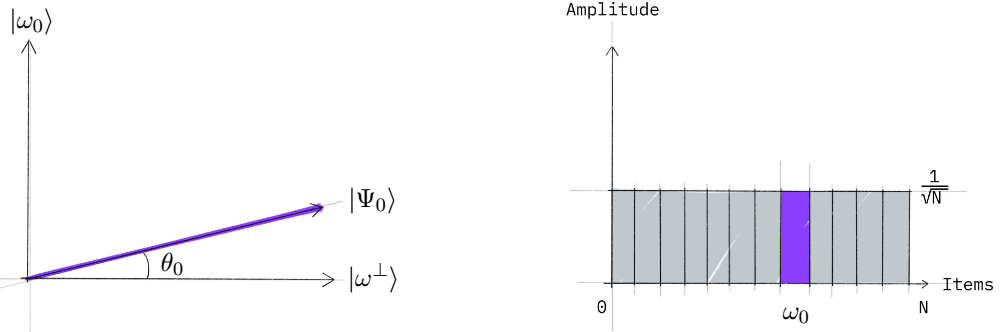
\includegraphics[width=0.85\linewidth]{Figuras/Fig_geo_1.png}
	\caption{Estado inicial del algoritmo de Grover: superposición uniforme de los $N$ estados. 
	En la figura de la izquierda, $| \Psi_0 \rangle$ representa el estado inicial, 
	el eje $|\omega_0 \rangle $ representa la solución y el eje $| \omega^{\perp} \rangle$ el resto de estados 
	de espacio de Hilbert. En la figura de la derecha vemos la \textbf{amplitud} de cada estado. 
	Recordemos que la probabilidad de cada estado es el cuadrado de la amplitud. Figura tomada 
	de \cite{Qiskit-Grover}.}
	\label{Fig_geo_1}
	\end{figure}

Sabemos también que todo vector en un plano podemos definirlo mediante su módulo y el ángulo respecto a uno de los ejes. Como el vector de estado tiene módulo uno (la suma de las probabilidades es uno), podemos escribirlo solo en función de un ángulo. Si llamamos $\theta_0$ al ángulo que forman el vector de estado con el eje $| \omega^{\perp} \rangle$, podemos escribir
\begin{equation} \label{ec_geo_theta}
| \Psi_0 \rangle = \sin \theta_0 \, |\omega_0 \rangle + \cos \theta_0 \, | \omega^{\perp} \rangle, \qquad \text{donde} \qquad  \boxed{\sin \theta_0 = \frac{1}{\sqrt{N}}}.
\end{equation}
En el gráfico de barras de la derecha en la Fig. \ref{Fig_geo_1} podemos ver las amplitudes de los estados. Recordemos que la probabilidad de un estado es el cuadrado de la amplitud.


\subsubsection{Primera parte de las iteraciones: El oráculo.}

El algoritmo de Grover usa un \textbf{oráculo} cuya función es aplicar una fase negativa al estado que buscamos, es decir
\begin{equation} \label{ec_geo_Uw}
\boxed{U_{\omega_0} | i \rangle = 
	\lch
		\begin{matrix}
			& | i \rangle \quad \text{si } i \neq \omega_0 \\
			& - | i \rangle \quad \text{si } i = \omega_0.
		\end{matrix}
	\right.}
\end{equation}

Este oráculo no es más que una matriz diagonal con todo 1 en la diagonal menos en el elemento correspondiente al estado $| \omega_0 \rangle$, donde tenemos un $-1$. Veremos más adelante ejemplos de como construir este tipo de oráculos. Podemos adelantar que, aunque no es trivial construirlos pues a priori parece que tenemos que conocer la solución de antemano, tampoco es (en muchos caso) excesivamente complicado. 

Una de las características importantes de este algoritmo es lo fácil que resulta convertir un problema a un oráculo de esta forma. Hay muchos problemas computacionales en los que es difícil encontrar una solución, pero relativamente fácil verificarla (problemas NP). Por ejemplo, podemos verificar fácilmente la solución de un sudoku comprobando que se cumplen todas las reglas. Para estos problemas, podemos crear una función $f$ que tome una propuesta de solución $i$ y nos devuelva $f(i)=0$ si $i$ no es solución ($i \neq  \omega_0$) y $f(i) = 1$ si $i$ es solución ($i \neq  \omega_0$). Podemos entonces definir el oráculo de la forma
\begin{equation} \label{ec_geo_U_f}
\boxed{U_{\omega_0} |i \rangle = (-1)^{f(i)} |i \rangle}.
\end{equation}
De esta forma, a matriz es ahora una matriz diagonal con 
\begin{equation}
Diag(U_{\omega_0})=\lc (-1)^{f(0)}, \, (-1)^{f(1)}, \dots , \, (-1)^{f(2^n-1)}    \rc .
\end{equation}

	\begin{mybox}{Nota}
	Podemos usar el retorno de fase (\textit{phase kickback}) para construir este tipo de oráculos. 
	Si tenemos nuestra función clásica $f(x)$,   podemos convertirla en un circuito reversible de la 
	forma (ver Fig. \ref{Fig_geo_phase_kick}(a))
	\begin{equation*}
	|x \rangle |0 \rangle \rightarrow |x \rangle | 0 \oplus f(x) \rangle  = |x \rangle | f(x) \rangle .
	\end{equation*}

	Si inicializamos la ancilla en el estado $| -\rangle$, tenemos (ver Fig. \ref{Fig_geo_phase_kick}(b))
	\begin{equation*}
	|x \rangle |- \rangle = \frac{1}{\sqrt{2}} |x \rangle \lp | 0 \rangle - | 1 \rangle \rp 
	\rightarrow 
	|x \rangle \lp | 0 \oplus f(x) \rangle - | 1 \oplus f(x) \rangle  \rp = (-1)^{f(x))} |x \rangle |- \rangle .
	\end{equation*} \vspace{-0.8cm}
	\begin{figure}[H] \setcounter{subfigure}{0}
	\centering
	\subfigure[]{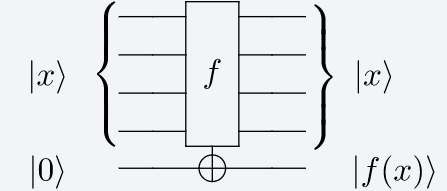
\includegraphics[width=0.3\linewidth]{Figuras/Fig_geo_phase_kick_0.png}} 
	\subfigure[]{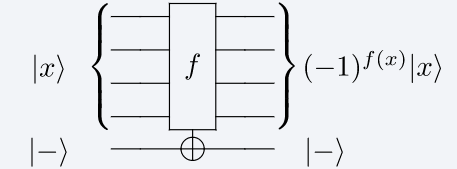
\includegraphics[width=0.35\linewidth]{Figuras/Fig_geo_phase_kick.png}}
	\caption{Retorno de fase (\textit{phase kickback}) para construir un oráculo de la forma de la 
	Ec. (\ref{ec_geo_U_f}). }
	\label{Fig_geo_phase_kick}
	\end{figure}

	\end{mybox}

En la Fig. \ref{Fig_geo_2} podemos ver el efecto del oráculo $U_{\omega_0}$ sobre el vector y las amplitudes. El cambio de signo en la amplitud del estado $| \omega_0 \rangle$ se traduce en un cambio de signo en la proyección del vector de estado sobre este eje. A efectos prácticos, esto no es más que una reflexíón del vector de estado respecto al eje $| \omega^{\perp} \rangle$. Como las probabilidades son el cuadrado de las amplitudes, este cambio de signo no se traduce en un cambio en la probabilidades. A efectos de las medidas, nada ha cambiado. En esta figura también se representa la media de las amplitudes (linea punteada). Vemos que ha disminuido la media al cambiar el signo de la amplitud del estado $| \omega_0 \rangle$. 

	\begin{figure}[H]
	\centering 
	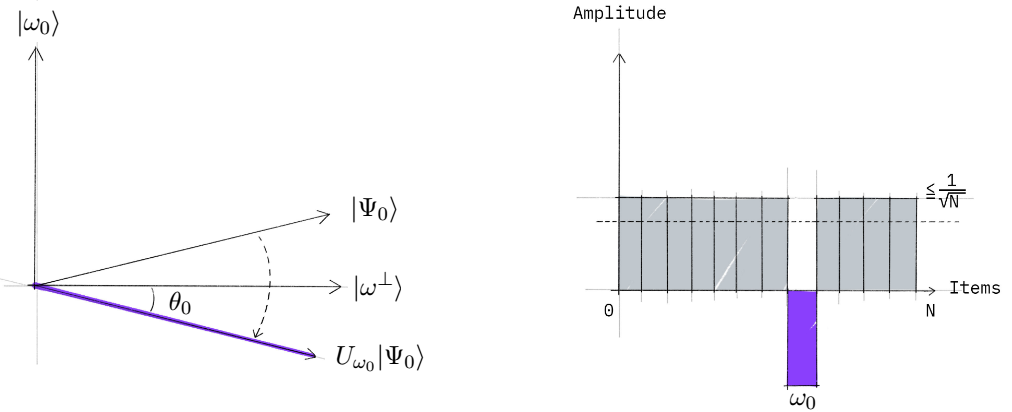
\includegraphics[width=0.85\linewidth]{Figuras/Fig_geo_2.png}
	\caption{Primer paso del algoritmo de Grover: aplicación del \textbf{oráculo} $U_{\omega_0}$ 
	para cambiar el signo de la amplitud del estado deseado. En la figura de la izquierda, 
	$| \Psi_0 \rangle$ representa el estado inicial, el eje $|\omega_0 \rangle $ 
	representa la solución y el eje $| \omega^{\perp} \rangle$ el resto de estados de espacio de Hilbert. 
	En la figura de la derecha vemos la \textbf{amplitud} de cada estado, donde la línea punteada 
	representa la media. Figura tomada de \cite{Qiskit-Grover}.}
	\label{Fig_geo_2}
	\end{figure}







\subsubsection{Segunda parte de las iteraciones: El difusor.}

El \textbf{difusor} consiste en aplicar el operador 
\begin{equation} \label{ec_geo_Us}
\boxed{U_{\Psi_0} = 2 |\Psi_0 \rangle \langle \Psi_0 | - I }.
\end{equation}
Este operador no es más que una reflexión respecto el esto inicial $|\Psi_0 \rangle$.


En la Fig. \ref{Fig_geo_3} podemos ver el efecto del difusor.  En el diagrama de barras de la amplitud, podemos entender esta transformación como una reflexión respecto a la media de las amplitudes (la media queda igual). Como habíamos disminuido la media al aplicar el oráculo, lo que tenemos ahora es una amplificación de la amplitud del estado deseado. Esto se ve también en el plano de la izquierda, pues las amplitudes no son más que las proyecciones del vector sobre los ejes. 

	\begin{figure}[t]
	\centering 
	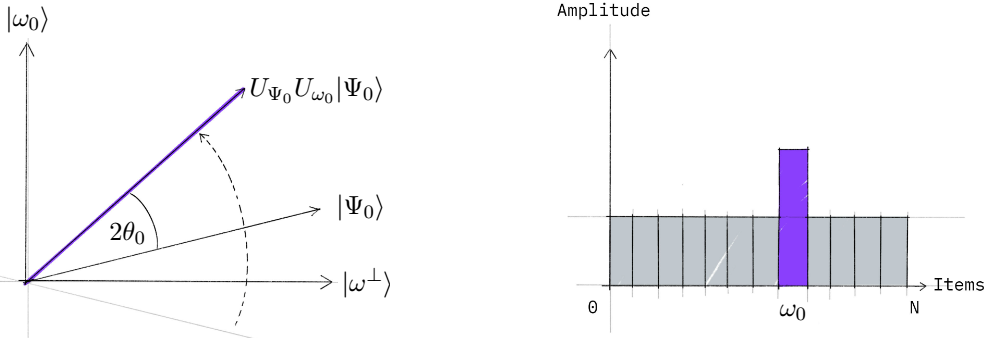
\includegraphics[width=0.85\linewidth]{Figuras/Fig_geo_3.png}
	\caption{Segundo paso del algoritmo de Grover: aplicar el operador de \textbf{difusión} 
	(o reflexión) $U_{\Psi_0} = 2 |\Psi_0 \rangle \langle \Psi_0 | - I$.  En la figura de la izquierda, 
	$| \Psi_0 \rangle$ representa el estado inicial, el eje $|\omega_0 \rangle $ representa 
	la solución y el eje $| \omega^{\perp} \rangle$ el resto de estados de espacio de Hilbert. En la figura de la 
	derecha vemos la \textbf{amplitud} de cada estado. Recordemos que la probabilidad de cada estado 
	es el cuadrado de la amplitud. Figura tomada de \cite{Qiskit-Grover}.}
	\label{Fig_geo_3}
	\end{figure}


Lo que estamos haciendo mediante la aplicación del oráculo y el difusor no es mas que \textbf{rotar el vector de estado un ángulo} $\bm{2 \theta_0}$ (donde $\theta_0$ está definido en la ec. (\ref{ec_geo_theta})) hacia el eje que representa nuestra solución, aumentando así su proyección, es decir, su amplitud, y con ello la probabilidad de medirlo. 

Después de $t$ iteraciones hemos aumentado el ángulo en $2t\theta_0$, con lo que tenemos estado:
\begin{equation} \label{ec_geo_phi-j}
\boxed{|\Psi(t) \rangle = \lp U_{\Psi_0} U_{\omega_0} \rp^t | \Psi_0 \rangle} = \sin \lp (2t+1) \theta_0 \rp \, |\omega_0 \rangle + \cos \lp (2t+1) \theta_0 \rp \, | \omega^{\perp} \rangle.
\end{equation}

Podemos ahora definir el \textbf{operador de Grover}
\begin{equation}
\boxed{G = U_{\Psi_0} U_{\omega_0}} \rqa |\Psi(t) \rangle =  G^t | \Psi_0 \rangle.
\end{equation}


Ahora es fácil entender porqué tenemos que aplicar un número concreto de iteraciones y porqué si nos pasamos, la probabilidad disminuye. Como acabamos de ver, el resultado después de cada iteración es que rotamos el vector de estado $2 \theta_0$ en el sentido contrario de las agujas del reloj. Lo que queremos es que el vector quede lo más vertical posible, es decir, que quede lo más cerca posible del eje $|\omega\rangle $. Si hacemos demasiadas iteraciones, lo que vamos a conseguir es ``pasarnos de largo'' del eje. Discutiremos el número exacto de iteraciones en la sección \ref{sec_t-sols}, pero ya comentamos que es del orden de $\sqrt{N}$.

Si comparamos las ecuaciones (\ref{ec_geo_phi-j-s}) y (\ref{ec_geo_phi-j}) vemos que
\begin{align} \label{ec_geo_sin-cos}
& \boxed{k(t) = \sin \Lc (2t+1) \theta_0 \Rc}
& \boxed{l(t) = \frac{1}{\sqrt{N-1}}\cos \Lc (2t+1) \theta_0 \Rc}.
\end{align}



\newpage
\section{Número conocido de soluciones.} \label{sec_t-sols}

Vamos a empezar el análisis formal tratando el caso en el que \textbf{conocemos el número $\bm M$ de soluciones} que hay en nuestro dataset. Es decir, tenemos $M$ valores diferentes $i$ que cumplen $L_i=x$. Denominemos $\omega$ al conjunto de los $M$ valores $i$ que son solución, y denominemos $\omega^\perp$ al conjunto de los $N-M$ valores $i$ que no son solución
\begin{align}
& \boxed{\omega = \lch i | L_{i} = x \rch }
& \boxed{\omega^{\perp} = \lch i | L_{i} \neq x \rch}.
\end{align}

Supondremos también que \textbf{estamos en el caso en el que} $N = 2^n$ y que además partimos del estado de la Ec. (\ref{ec_geo_phi-0_1}), es decir, de una \textbf{superposición uniforme}. 

	\begin{mybox}{Nota Importante!!}
	Uno de los pasos del algoritmo de Grover es una reflexión de las amplitudes respecto a la media. 
	Esto implica que podemos tener los siguientes casos:
	\begin{itemize}
		\item $M < N/2$: El algoritmo funciona normal.
		
		\item $M = N/2$: El algoritmo no funciona
		
		\item $M > N/2$: El algoritmo amplifica las soluciones incorrectas.
	\end{itemize}
	\end{mybox}

\subsection{Generalización de las expresiones de la sección \ref{sec_geo} para $M$ soluciones.}

Vemos a reescribir las ecuaciones enmarcadas de la sección \ref{sec_geo} para el caso de $M$ soluciones. Empecemos reescribiendo las expresiones del estado inicial de la Ec. (\ref{ec_geo_phi-0_2}) y del estado $|\Psi_j \rangle $ de la Ec. (\ref{ec_geo_phi-j}) 
\begin{equation} \label{ec_t-sols_phi-0}
\boxed{|\Psi_0 \rangle = | \Psi (k(0),l(0)) \rangle = \sum_{i \in \omega} k(0) |i \rangle + \sum_{i  \in \omega^{\perp}}  l(0)  |i \rangle}, \quad \text{donde} \quad \boxed{k(0) = l(0) = \frac{1}{\sqrt{N}}}.
\end{equation}
\begin{equation} \label{ec_t-sols_phi-j}
\boxed{|\Psi(t) \rangle = | \Psi (k(t),l(t)) \rangle = \sum_{i \in \omega} k(t) |i \rangle + \sum_{i  \in \omega^{\perp}} l(t) |i \rangle }.
\end{equation}
Vemos que ahora el primer sumatorio tiene $M$ elementos, mientras que el segundo tiene $N-M$. Por supuesto, se cumple que $|\Psi(t) \rangle$ tiene módulo 1, es decir
\begin{equation} \label{ec_t-sols_mod_1}
\langle \Psi(t) |\Psi(t) \rangle = \boxed{ M k(t)^2 + (N-M) l(t)^2 = 1 \, \, \forall t}.
\end{equation}
Podemos ahora también redefinir el estado $|\omega^{\perp} \rangle$ de la Ec. (\ref{ec_geo_phi-j-s}) y definir $| \omega \rangle$
\begin{align} \label{ec_t-sols_omega_omega-perp}
& \boxed{| \omega^{\perp}  \rangle = \frac{1}{\sqrt{N-M}}\sum_{i \in \omega^{\perp}}  |i \rangle}
& \boxed{| \omega  \rangle = \frac{1}{\sqrt{M}}\sum_{i \in \omega} | i \rangle}
\end{align}
de forma que
\begin{equation} \label{ec_t-sols_phi-j-s}
\boxed{|\Psi(t) \rangle =  k(t) \sqrt{M} |\omega \rangle + l(t) \sqrt{N-M} | \omega^{\perp}  \rangle}.
\end{equation}

	\begin{mybox}{Nota}
	Nuevamente, los factores $\sqrt{N-M}$ y $\sqrt{M}$ en las definiciones de $| \omega^{\perp} \rangle$ y $| \omega \rangle$ son para hacerlos vectores unitarios
	\begin{align}
	& \langle \omega^{\perp} | \omega^{\perp} \rangle = 1 
	& \langle \omega | \omega \rangle = 1 .
	\end{align}
	\end{mybox}

Veamos ahora la expresión del esto inicial en función del ángulo $\theta$ de la Ec. (\ref{ec_geo_theta})
\begin{equation} \label{ec_t-sols_theta}
| \Psi_0 \rangle = \sin \theta \, |\omega \rangle + \cos \theta \, | \omega^{\perp} \rangle, \qquad \text{donde} \qquad  \boxed{\sin \theta = \sqrt{\frac{M}{N}}}.
\end{equation}
Nuevamente, comparando las Ecs. (\ref{ec_t-sols_theta}) y (\ref{ec_t-sols_phi-j-s}) obtenemos las expresiones de $k(t)$ y $l(t)$ en función del ángulo $\theta$
\begin{align} \label{ec_t-sols_sin-cos}
& \boxed{k(t) = \frac{1}{\sqrt{M}} \sin \Lc (2t+1) \theta \Rc}
& \boxed{l(t) = \frac{1}{\sqrt{N-M}}\cos \Lc (2t+1) \theta \Rc}.
\end{align}
Vemos que estas expresiones cumplen la Ec. (\ref{ec_t-sols_mod_1}) 
Finalmente, por ser rigurosos (y por recopilar todas las ecuaciones juntas), tenemos que el oráculo (\ref{ec_geo_Uw}), el difusor (\ref{ec_geo_Us}) nos quedan:
\begin{align} \label{ec_t-sols_Uw_Us}
& \boxed{U_\omega | i \rangle = 
	\lch
		\begin{matrix}
			& | i \rangle \quad \text{si } i \not \in \omega \\
			& - | i \rangle \quad \text{si } i \in \omega
		\end{matrix}
	\right.}
& \boxed{U_{\Psi_0} = 2 |\Psi_0 \rangle \langle \Psi_0 | - I}.
\end{align}
donde recordemos que denominamos operador de Grover a
\begin{equation} \label{ec_t-sols_G}
\boxed{G = U_{\Psi_0} U_\omega} \rqa |\Psi(t) \rangle =  G^t | \Psi_0 \rangle.
\end{equation}

Véase que el caso particular de una solución es, efectivamente, aquel con $M=1$.

\subsection{Número de iteraciones.}

Denominemos $\bm T$ al \textbf{número de iteraciones para el cual la probabilidad de medir la solución correcta se maximiza}. Es decir, $l(T) \approx 0$ y $k(T) \approx 1$. Sabemos que $l(\tilde{T}) =0$ cuando el coseno es igual cero, es decir:
\begin{equation}
l(\tilde{T}) = 0 \rqa (2\tilde{T}+1) \theta = \frac{\pi}{2} \rqa \tilde{T} = \frac{\pi}{4 \theta} - \frac{1}{2}.
\end{equation}
Por regla general, este valor $\tilde{T}$ no será un entero. Tomemos 
\begin{equation} 
T = \lfloor \pi / 4 \theta \rfloor
\end{equation}
donde la notación $\lfloor \alpha \rfloor$ quiere decir que \textbf{redondeamos a un entero por truncamiento}. Véase que $|m-\tilde{m}| \leq 1/2$. Se sigue que $|(2T+1)\theta - (2\tilde{T}+1)\theta | \leq \theta $. Pero $(2 \tilde{T}+1) \theta = \pi/2$ por definición de $\tilde{T}$. Con lo cual $\left| \cos \Lp (2T+1) \theta \Rp \right| \leq | \sin \theta |$. Concluimos entonces que la probabilidad de fallo después de $T = \lfloor \pi / 4 \theta \rfloor$ es 
\begin{equation}
(N-M)l^2(T) = \cos^2 \Lp (2T+1) \theta \Rp \leq \sin^2 \theta = \frac{M}{N}
\end{equation}
que es despreciable si $M \ll N$. Véase que el $(N-M)$ de la expresión anterior es porque hay $(N-M)$ estados incorrectos que podemos medir, cada uno de ellos con probabilidad $l^2(T)$.

Véase que el algoritmo corre en un tiempo del orden de $\mathcal{O}(\sqrt{N/M})$ ya que
\begin{equation} \label{ec_t-sols_m}
T \leq \frac{\pi}{4 \theta} \approx \frac{\pi}{4 \sin \theta} \approx \frac{\pi}{4} \sqrt{\frac{N}{M}} \rqa \boxed{T = \left\lfloor \frac{\pi}{4} \sqrt{\frac{N}{M}} \right\rfloor}.
\end{equation}


\subsection{Extra: Formulación recursiva de $k(t)$ y $l(t)$.}

Ya hemos comentado en cada iteración se aplican lo dos operadores de la Ec. (\ref{ec_t-sols_Uw_Us}), es decir
\begin{equation} \label{ec_t-sols_Psi_j+1_j}
|\Psi{(t+1)} \rangle = U_{\Psi_0} U_\omega |\Psi(t) \rangle.
\end{equation}

Desarrollemos esta expresión para ver la relación de recursivida de los coeficientes, es decir, para ver la expresión de $k(t+1)$ y $l(t+1)$ en función de $k(t)$ y $l(t)$. Primero vamos el término $U_\omega |\Psi(t) \rangle$ usando la expresión de $U_\omega$ de la Ec. (\ref{ec_t-sols_Uw_Us}):
\begin{equation} \label{ec_t-sols_aux_1}
U_\omega |\Psi(t) \rangle =  - k(t)  \sqrt{M}|\omega \rangle + l(t) \sqrt{N-M} | \omega^{\perp} \rangle.
\end{equation}

Desarrollemos un poco la Ec. (\ref{ec_t-sols_Psi_j+1_j}) usando la expresión de $U_{\Psi_0}$ de la  Ec. (\ref{ec_t-sols_Uw_Us})
\begin{equation} \label{ec_t-sols_aux_2}
\begin{split}
|\Psi(t+1) \rangle & =  U_{\Psi_0} U_\omega |\Psi(t) \rangle  \\
& =  \Bigl( 2 |\Psi_0 \rangle \langle \Psi_0 | - I \Bigr) U_\omega |\Psi(t) \rangle  \\ 
& =  2 |\Psi_0 \rangle \langle \Psi_0 |  U_\omega |\Psi(t) \rangle  - U_\omega |\Psi(t) \rangle .
\end{split}
\end{equation}

Usando la Ec. (\ref{ec_t-sols_aux_1}) el término $\langle \Psi_0 |  U_\omega |\Psi(t) \rangle$ nos queda
\begin{equation} \label{ec_t-sols_aux_3}
\langle \Psi_0 | U_\omega |\Psi(t) \rangle = \frac{1}{\sqrt{N}} \Lp -k(t) M + (N-M) l(t) \Rp.
\end{equation}

	\begin{mybox_green}{Calculo de $\langle \Psi_0 |  U_\omega |\Psi(t) \rangle$}
	Hacemos ahora el producto $ \langle \Psi_0 |  U_\omega |\Psi(t) \rangle  =  \langle \Psi_0 | \Lp U_\omega |\Psi(t) \rangle \Rp $ 
	usando la Ec. (\ref{ec_t-sols_aux_1})
	\begin{equation*}
	\begin{split}
	\langle \Psi_0 | U_\omega |\Psi(t) \rangle 
	& = \langle \Psi_0 | \Lp -k(t) \sqrt{M} |\omega \rangle + l(t) \, \sqrt{N-M} | \omega^{\perp} \rangle \Rp \\
	& = \Lp k(0) \sqrt{M} \langle \omega| + l(0) \, \sqrt{N-M} \langle \omega^{\perp} | \Rp
	\Lp -k(t) \sqrt{M} |\omega \rangle + l(t) \, \sqrt{N-M} | \omega^{\perp} \rangle \Rp .
	\end{split}
	\end{equation*}
	Debido a la ortogonalidad de los estado (esto es, $\langle i | j \rangle =0$ si $j\neq i$), y teniendo en cuanta que $k(0) = l(0) = 1/\sqrt{N}$ tenemos
	\begin{equation*} 
	\langle \Psi_0 | U_\omega |\Psi(t) \rangle = - k(0) k(t) M + (N-M) l(0) l(t) = 
	\frac{1}{\sqrt{N}} \Lp -k(t) M + (N-M) l(t) \Rp.
	\end{equation*}
	\end{mybox_green}	

Sustituyendo (\ref{ec_t-sols_aux_1}) y (\ref{ec_t-sols_aux_3}) en (\ref{ec_t-sols_aux_2}) tenemos:
\begin{equation} \label{ec_t-sols_aux_4}
|\Psi(t+1) \rangle  = \lp \frac{N-2M}{N} k(t) + \frac{2(N-M)}{N} l(t) \rp \sum_{i \in \omega} | i \rangle + \lp \frac{N-2M}{N} l(t) - \frac{2M}{N} k(t) \rp \sum_{i \in \omega^{\perp}} | i \rangle.
\end{equation}
	
	\begin{mybox_green} {Calculo de la Ec. (\ref{ec_t-sols_aux_4})}
	Sustituyendo (\ref{ec_t-sols_aux_1}) y (\ref{ec_t-sols_aux_3}) en (\ref{ec_t-sols_aux_2}) tenemos:
	\begin{align*}
	|\Psi (t+1) \rangle & = 
	\, 2  \frac{1}{\sqrt{N}} \Lp -k(t) M + (N-M) l(t) \Rp | \Psi_0 \rangle 
	- k(t) \sqrt{M} |\omega \rangle +  l(t) \, \sqrt{N-M} | \omega^{\perp} \rangle  = \\
	& =  \, \frac{2}{\sqrt{N}} \Lp -k(t) M + (N-M) l(t) \Rp  \frac{1}{\sqrt{N}} \Lp \sqrt{M} | \omega \rangle + \sqrt{N-M} |\omega^{\perp} \rangle \Rp \\ 
	& \qquad + k(t) \sqrt{M} |\omega \rangle  +   l(t) \, \sqrt{N-M} | \omega^{\perp} \rangle = \\
	& =  \, \lc \frac{2}{N} \Lp -k(t) M + (N-M) l(t) \Rp + k(t) \rc \sqrt{M}  | \omega \rangle   \\
	& \qquad + \lc \frac{2}{N}  \Lp -k(t) M + (N-M) l(t) \Rp - l(t)  \rc \sqrt{N-M} | \omega^{\perp} \rangle.
	\end{align*}
	Simplificando y teniendo en cuenta que las expresión de $| \omega \rangle$ y $|\omega^{\perp} \rangle$ en la 
	Ec. (\ref{ec_t-sols_omega_omega-perp}), llegamos a la Ec. (\ref{ec_t-sols_aux_4}).
	\end{mybox_green}

Finalmente llegamos a las relaciones:
\begin{align} \label{ec_t-sols_k-l_j+1}
& \boxed{k(t+1) = \frac{N-2M}{N} k(t) + \frac{2(N-M)}{N} l(t)},
& \boxed{l(t+1) = \frac{N-2M}{N} l(t) - \frac{2M}{N}k(t)}.
\end{align}
%No es difícil comprobar que estas relaciones se cumplen si tomamos las expresiones de la Ec. (\ref{ec_t-sols_sin-cos}).



\newpage
\section{Número desconocido de soluciones} \label{sec_t_no_conocido}

Como ya hemos comentado, para poder aplicar el algoritmo de Grover tal y como lo hemos visto hasta ahora, nos hace falta conocer el número de soluciones. Esto es debido a que debemos aplicar un número concreto de iteraciones para maximizar la probabilidad de las soluciones correctas. Si no aplicamos el número correcto de iteraciones, la probabilidad puede ser incluso nula. Como vemos en la Ec. (\ref{ec_t-sols_m}), para saber el número de iteraciones tenemos que conocer el número de soluciones. 

En esta sección vamos a ver un algoritmo para poder abordar el caso en el que no conocemos el número de soluciones y por ende, no sabemos cuantas iteraciones debemos aplicar. Este algoritmo no es más que una forma inteligente de aplicar el algoritmo de Grover. Lo bueno de este algoritmo es que nuevamente podemos encontrar una solución con un número de iteraciones $\mathcal{O}( \sqrt{N/M} )$, aunque a priori no sabemos cuantas iteraciones son. Vamos a ver primero dos Lemmas que nos servirán para entender el algoritmo que se plantea en el Teorema \ref{teorema_no-t}.

	\begin{mybox}{Nota Importante!!}
	Uno de los pasos del algoritmo de Grover es una reflexión de las amplitudes respecto a la media. 
	Esto implica que podemos tener los siguientes casos:
	\begin{itemize}
		\item $M < N/2$: El algoritmo funciona normal.
		
		\item $M = N/2$: El algoritmo no funciona
		
		\item $M > N/2$: El algoritmo amplifica las soluciones incorrectas.
	\end{itemize}
	\end{mybox}


\subsection{Conocimientos previos.}

\begin{lemma}  \label{lemma_suma_cos}
Para cualquier par de números $\alpha$ y $\beta$, y cualquier posible entero $r$ tenemos
\begin{equation}
\sum_{j=0}^{r-1} \cos \lp \alpha + 2 \beta j \rp = \frac{\sin \lp r \beta \rp \cos (\alpha + (r-1) \beta)}{\sin \beta}.
\end{equation}
En particular, si $\alpha = \beta$,
\begin{equation}
\sum^{r-1}_{j=0} \cos \lp \lp 2 j + 1 \rp \alpha \rp = \frac{\sin \lp 2 r \alpha \rp}{2 \sin \alpha}.
\end{equation}
\end{lemma}

\begin{lemma} \label{lemma_Pm}
Sea $M$ el número (desconocido) de soluciones de un problema tipo Grover con $N$ elementos y sea $\theta$ tal que $\sin^2 \theta = M/N$. Sea $r$ un entero positivo aleatorio. Sea $t$ un entero aleatorio (con distribución uniforme) entre $0$ y $r-1$. Si observamos el registro después de $t$ iteraciones del algoritmo de Grover empezando desde el estado $|\Psi_0 \rangle = \sum_i \frac{1}{\sqrt{N}} | i \rangle$, la probabilidad de obtener la solución correcta es exactamente 
\begin{equation} \label{lemma_Pm_ec}
P_r = \frac{1}{2} - \frac{\sin (4 r \theta)}{4 r \sin(2 \theta)}.
\end{equation}
En particular, tenemos $P_r \geq 1/4$ si $r \geq 1/\sin ( 2 \theta)$.
\end{lemma}


\begin{proof}
 Como ya sabemos, si tenemos $M$ soluciones la probabilidad de que tras $t$ iteraciones se mida el resultado correcto es $M$ veces el valor del coeficiente $k^2(t)$ (la amplitud al cuadrado del estado $i \in \omega$ en la Ec. (\ref{ec_t-sols_Psi_j+1_j})). Teniendo en cuenta la Ec. (\ref{ec_t-sols_k-l_j+1}) sabemos que la probabilidad es
\begin{equation*}
P(t) = M k^2(t) = \sin^2 ((2t+1)\theta).
\end{equation*}
De esto se sigue que la probabilidad promedio si tomamos un número de iteraciones $t$ tal que $0 \leq t < r$ es
\begin{equation*}
P_r = \frac{1}{r} \sum^{r-1}_{t=0}  P(t) = \frac{1}{r} \sum^{r-1}_{t=0} \sin^2 ((2t+1) \theta) = 
\frac{1}{2r} \sum^{r-1}_{t=0} \Lp 1-\cos ((2t+1) \theta) \Rp = \frac{1}{2} - \frac{\sin (4 r \theta)}{4 r \, \sin (2 \theta)},
\end{equation*}
donde en la última igualdad se ha usado el Lemma \ref{lemma_suma_cos}. Si estamos en el caso de $r \geq 1/\sin (2\theta)$ tenemos
\begin{equation*}
\frac{\sin (4 r \theta)}{4 r \, \sin (2 \theta)} \leq \frac{1}{4 r \, \sin (2 \theta)} \leq \frac{1}{4} \rqa P_r \geq \frac{1}{2} - \frac{1}{4},
\end{equation*}
donde la primera desigualdad se cumple siempre (independientemente del valor de $r$) pues viene de que la función seno está acotada entre $-1$ y $1$.
\end{proof}


	\begin{mybox}{Nota}
	A veces al ver las formulaciones tan formales que se dan en los teoremas o lemmas, perdemos un poco el 
	norte sobre lo que nos quieren transmitir. Veámoslos en palabras más llanas:
	\begin{itemize}
		\item El Lemma \ref{lemma_suma_cos} simplemente es una relación trigonométrica un poco exótica y nos
		 sirve para demostrar el Lemma \ref{lemma_Pm}

		\item El Lemma \ref{lemma_Pm} nos da la expresión de la probabilidad promedio que tenemos de medir el 
		resultado correcto usando el algoritmo de Grover en un caso particular. En este caso lo que hacemos es, 
		dado un número $r$, ejecutar $t$ iteraciones de Grover donde $t$ es un número aleatorio  entre $0$ y 
		$r-1$. Probando muchas veces con muchos número aleatorio $t$, en promedio la probabilidad 
		$P_r$ de obtener el resultado correcto está dada por (\ref{lemma_Pm_ec}). Véase que, para un problema de 
		Grover concreto ($\theta$ fijo), esta probabilidad depende solo de $r$. 
	\end{itemize}
	\end{mybox}

\subsection{Algoritmo para el caso de $M$ desconocido.}

\begin{theorem} \label{teorema_no-t}
El siguiente algoritmo encuentra una solución en un tiempo esperado $\mathcal{O} ( \sqrt{N/M} )$ (si tomamos $1 \leq M \leq 3N/4$)
\begin{enumerate}
\item Inicializamos $r=1$ y $\lambda = 6/5$. (En realidad, cualquier valor $1 \leq \lambda \leq 4/3$ sirve).

\item Elegimos un valor aleatorio $t$ con distribución uniforme tal que $0 \leq t < r$.

\item Aplicamos $t$ iteraciones del algoritmo de Grover empezando desde el estado inicial $| \Psi_0 \rangle = \sum_i \frac{1}{\sqrt{N}} |i \rangle$.

\item Medimos, de forma que obtenemos uno de los estados $|i \rangle$ del paso anterior. 

\item Si $L_i = x$, hemos encontrado una solución:  \textbf{Exit}.

\item En caso contrario, tomemos $r = $ min$(\lambda r, \sqrt{N})$ y volvemos al paso 2.
\end{enumerate}
\end{theorem}


\subsection{Demostración del Teorema \ref{teorema_no-t}.}

\begin{proof}
Sea $\theta$ un ángulo tal que 
\begin{equation} \label{teorema_no-t_proof_theta}
\sin \theta = \sqrt{N/M},
\end{equation}
(como en la Ec. (\ref{ec_t-sols_theta})). Denominemos $r_s$ al valor de $r$ en la s-esima iteración del bucle principal, es decir
\begin{equation} \label{teorema_no-t_proof_r-s}
r_s = \lambda^{s-1}, \qquad \text{con } s = 1,2,\dots \quad \text{ y } \lambda = \frac{4}{3}.
\end{equation} 
(No confundir las \textbf{iteraciones del bucle principal} con las \textbf{iteraciones de Grover}: en cada iteración $s$ del bucle principal hacemos $t$ iteraciones de Grover.) Sea $r_0$ tal que
\begin{equation}  
r_0 = \frac{1}{\sin (2 \theta)}.
\end{equation}
(Véase que $r_0$ no es valor inicial de $r_s$). Aplicando un poco de trigonometria
\begin{equation*}
\sin^2 \theta =  \frac{1-\cos (2\theta)}{2} 
\rqa 1 - 2 \sin^2 \theta = \cos (2 \theta) = \sqrt{1 - \sin^2 (2 \theta)} 
\rqa \sin^2 (2 \theta) = 1 - \Lp 1 - 2 \sin^2 \theta \Rp^2.
\end{equation*}
Desarrollando el cuadrado y teniendo en cuenta la Ec. (\ref{teorema_no-t_proof_theta}) llegamos a
\begin{equation} \label{teorema_no-t_proof_alpha}
r_0 = \frac{1}{\sin (2 \theta)} = \frac{N}{2 \sqrt{(N-M)M}} < \sqrt{\frac{N}{M}}.
\end{equation}
donde en la desigualdad se ha tenido en cuenta que $M \leq 3N/4$. Veámoslo
\begin{align*}
\frac{N}{2 \sqrt{(N-M)M}} < \sqrt{\frac{N}{M}} 
\rqa  \frac{\sqrt{N}}{2 \sqrt{(N-M)}} < 1 
\rqa \frac{N}{(N-M)} < 4 
\rqa  1 - \frac{1}{4} > \frac{M}{N}.
\end{align*}

Debemos estimar el número esperado total de iteraciones de Grover que tenemos que hacer (sumando todas las interaciones de Grover en todas las iteraciones del bucle principal). El tiempo total será del orden de este número. Sabemos que \textbf{el número promedio de iteraciones de Grover que se realizan en la iteración s-esima del bucle principal es menor que} $\bm{r_s/2}$. Escribiéndolo de forma bonita:
\begin{equation} \label{teorema_no-t_proof_j-hat}
\bar{t}_s < \frac{r_s}{2} = \frac{\lambda^{s-1}}{2} \qquad \text{ donde la barra significa \textit{promedio}}.
\end{equation} 
Esto es debido a que en cada iteración del bucle principal hacemos un número aleatorio de iteraciones $t_s$ de Grover con $0 \leq t_s < r_s$.  Denominamos \textbf{fase crítica} al momento en el que hemos realizado suficientes iteraciones del bucle principal como para tener $r_s \geq r_0$, es decir
\begin{equation} 
r_s > r_0 \rqa \lambda^{s-1} > r_0 \rqa s > 1 + \log_{\lambda} r_0  \rqa s > \lceil \log_\lambda r_0 \rceil.
\end{equation}
con lo cual, \textbf{estamos en la fase crítica cuando el número de iteraciones del bucle principal es mayor que} $\bm{\lceil \log_{\lambda} r_0 \rceil}$ (donde esta notación significa \textit{redondear hacia el siguiente entero}).  Si nos fijamos en el Lemma \ref{lemma_Pm}, esta fase corresponde a aquella donde $P_r > 1/4$.

Teniendo en cuenta la Ec. (\ref{teorema_no-t_proof_j-hat}), vemos que el número promedio total de iteraciones de Grover que se realizan antes de llegar a la fase crítica es
\begin{equation} \label{teorema_no-t_3r0}
\begin{split}
\sum_{s=1}^{\lceil \log_\lambda r_0 \rceil} \bar{t}_s 
& = \frac{1}{2} \sum_{s=1}^{\lceil \log_\lambda r_0 \rceil} \lambda^{s-1} 
= \frac{1}{2} \sum_{\tilde{s}=0}^{\lceil \log_\lambda r_0 \rceil-1} \lambda^{\tilde{s}}  = \frac{1}{2} \frac{ \lambda^{\lceil \log_\lambda r_0 \rceil} -1 }{\lambda -1 }  < \\
& < \frac{1}{2} \frac{\lambda^{1 + \log_\lambda r_0} -1 }{\lambda -1} = \frac{1}{2} \frac{r_0 \lambda -1 }{\lambda  -1 }  < 
 \frac{1}{2} \frac{\lambda}{\lambda - 1} r_0 = \boxed{3 r_0}.
\end{split}
\end{equation}

donde se ha aplicado la formula e la suma de la serie geométrica\footnote{Suma de la serie geométrica: \begin{equation} \label{ec_no-t_suma-geometrica}
\sum_{k=0}^n r^k = \frac{1-r^{n+1}}{1-r} = \frac{r^{n+1} -1 }{r -1}.
\end{equation}}. 
Vemos pues que el algoritmo llega a la fase crítica en un tiempo $\mathcal{O} (r_0) < \mathcal{O}(\sqrt{N/M})$. 

Como ya comentamos, una vez alcanzado el estado crítico, por el Lemma \ref{lemma_Pm}, sabemos que en cada nueva iteración del bucle principal la \textbf{probabilidad de éxito} $\bm{P_r \geq 1/4}$ ya que $r_s > 1/\sin (2 \theta)$. De ello se deduce que el número esperado de iteraciones de Grover necesarias para tener éxito una vez alcanzada la fase crítica está acotado superiormente por
\begin{equation}
\sum_{\tilde{u}=1}^\infty (1-P_r)^{\tilde{u}-1} P_r \, \bar{t}_{\tilde{u}+1+\lceil \log_\lambda r_0 \rceil} < \frac{1}{2} \sum_{\tilde{u}=1}^\infty \frac{3^{\tilde{u}-1}}{4^{\tilde{u}-1}} \frac{1}{4} \lambda^{\tilde{u}+1+\lceil \log_\lambda r_0 \rceil},
\end{equation}
donde $(1-P_r)^{\tilde{u}-1}$ es la probabilidad de fallar $\tilde{u}-1$, con lo que $(1-P_r)^{\tilde{u}-1} P_r$ es la probabilidad de haber fallado $\tilde{u}-1$ veces y acertar en la $\tilde{u}$-esima. $\bar{t}_s$ viene dada por (\ref{teorema_no-t_proof_j-hat}). Véase que para acotar las iteraciones nos hemos puesto en el peor caso, en el que la probabilidad de exito es la mínima y no aumenta ($P_r = 1/4$). Podemos hacer al cambio de variable $u = \tilde{u} -1$ para poner la expresión anterior más acorde para realizar la suma de la serie geométrica (ver Ec. (\ref{ec_no-t_suma-geometrica}))
\begin{equation} \label{teorema_no-t_3r0/2}
\frac{1}{2} \sum_{u=0}^\infty \frac{3^{u}}{4^{u}} \frac{1}{4} \lambda^{u+\lceil \log_\lambda r_0 \rceil} 
< 
\frac{1}{2}  \frac{1}{4} \lambda^{1+ \log_\lambda r_0}  \sum_{u=0}^\infty \frac{3^{u}}{4^{u}} \lambda^{u} 
= 
\frac{r_0 \lambda}{8} \frac{1}{1-3 \lambda/4} 
= \frac{\lambda}{8-6 \lambda}r_0 = \boxed{ \frac{3}{2} r_0}.
\end{equation}
El número total esperado de iteraciones de Grover, en caso de que se alcance la fase crítica, está, por tanto, limitado por la suma de (\ref{teorema_no-t_3r0}) más (\ref{teorema_no-t_3r0/2}), es decir, 
\begin{equation}
T = r_0 + \frac{3}{2} r_0 = \frac{9}{2} r_0 < \frac{9}{2} \sqrt{\frac{M}{N}},
\end{equation}  
con lo que el tiempo esperado total es $\mathcal{O}(\sqrt{N/M})$ siempre que $0 < M \leq 3N/4$. Véase que $\frac{9}{2} r_0 \approx \frac{9}{2} \sqrt{N/M}$ cuando $M \ll N$, que es menos de 4 veces el tiempo esperado en el caso de conocer $M$ de antemano (ver Ec. (\ref{ec_t-sols_m})). El caso $M > 3N/4$ puede resolverse en tiempo esperado constante mediante muestreo clásico. El caso $M = 0$ se maneja mediante un tiempo de espera apropiado en el algoritmo anterior, que permite afirmar en un tiempo en $\mathcal{O} (\sqrt{N})$ que no hay soluciones cuando este es el caso, con una probabilidad de fallo arbitrariamente pequeña cuando de hecho hay una solución.
\end{proof}






\newpage
\section{Conteo de soluciones (Quantum counting)} \label{sec_quantum_counting}


En esta sección vamos a ver un algoritmo para obtener el número $M$ de soluciones. Este algoritmo puede decirse que en cierta medida está inspirado en el algoritmo de Shor, pues lo que vamos a hacer es usar el \textbf{algoritmo de estimación de fase cuántico (QPE)} para obtener el ángulo $\theta$ a partir del operador de Grover $G$. Después, podemos usar la Ec. (\ref{ec_t-sols_theta}) para obtener $M$ partir de $\theta$.

Vamos a seguir en el caso en el que $N=2^n$ y la distribución de probabilidad inicial es uniforme.

\subsection{Breve resumen de la estimación de fase cuántica (QFE).}

Dado un operador unitario $U$ y un autovector $\left| \psi \right\rangle$ del mismo, tenemos:
$$
U \left| \psi \right\rangle = e^{2 \pi i \alpha}  \left| \psi \right\rangle
$$
El \textbf{algoritmo de estimación de fase cuántica} lo que hace es calcular un valor aproximado del ángulo $\alpha$.
En la Fig. \ref{Fig_QC_QPE} podemos ver el circuito que implementa este algoritmo. No vamos a entrar a hablar en detalle del mismo (puede verse una explicación más detallada en las notas del algoritmo de Shor). Simplemente comentar dos cosas:
\begin{itemize}
	\item Por el registro de qubits de abajo en la Fig. \ref{Fig_QC_QPE} debe de entrar el autoestado de $U$ del cual queremos medir la fase.
	
	\item Si por el registro de conteo entran $p$ qubits (el de arriba en la Fig. \ref{Fig_QC_QPE}), en la salida vamos a medir el estado $| 2^p \alpha \rangle$.
\end{itemize}

	\begin{figure}[h] 
	\centering 
	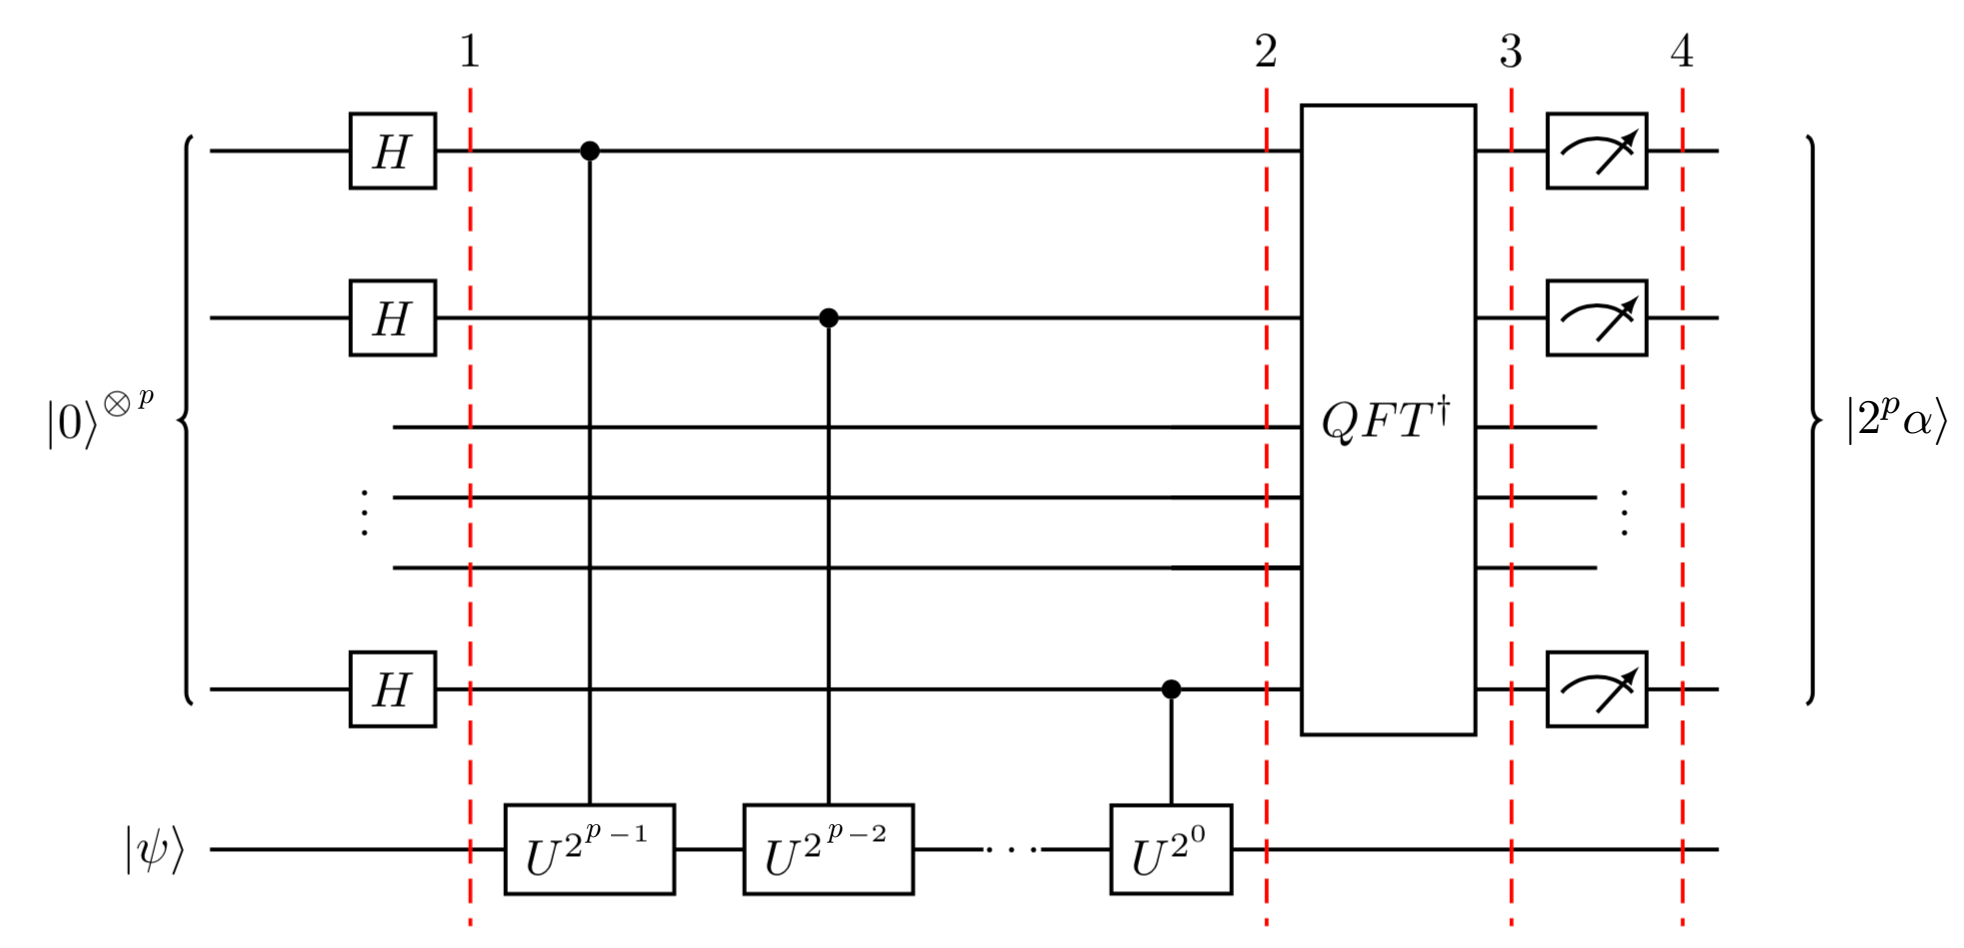
\includegraphics[width=0.8\linewidth]{Figuras/Fig_QC_QPE.png}
	\caption{Implementación del algoritmo de estimación de fase cuántica 
	(en el convenio estándar, siendo el bit más significativo el de arriba).}
	\label{Fig_QC_QPE}
	\end{figure}

\subsection{Estimación de fase con el operador de Grover.}

Como ya comentamos anteriormente, el operador de Grover $G$ (ver Ec. (\ref{ec_t-sols_G})) rota el vector de estado en un ángulo $2\theta$, donde $\theta$ está dado por (\ref{ec_t-sols_theta}), es decir
\begin{equation}
|\Psi(t+1) \rangle = G | \Psi(t) \rangle = e^{i 2 \theta} | \Psi(t) \rangle.
\end{equation}
En concreto, se puede aplicar sobre el estado inicial
\begin{equation}
\boxed{G | \Psi_0 \rangle = e^{i 2 \theta} | \Psi_0 \rangle}, 
\qquad \text{ donde } \qquad
| \Psi_0 \rangle = H^{\otimes n} |0\rangle = \frac{1}{2^n}  \sum_{i=0}^{2^n} | i \rangle
\end{equation}
Podemos pues usar el algoritmo de QFE poniendo el registro de abajo en el estado $| \Psi_0 \rangle $ y mediremos a la salida el estado $| 2^p 2 \theta / 2 \pi \rangle = | 2^p \theta / \pi \rangle$. Podemos ver esto en la Fig. \ref{Fig_QC_QPE_G}.

	\begin{figure}[h]
	\centering 
	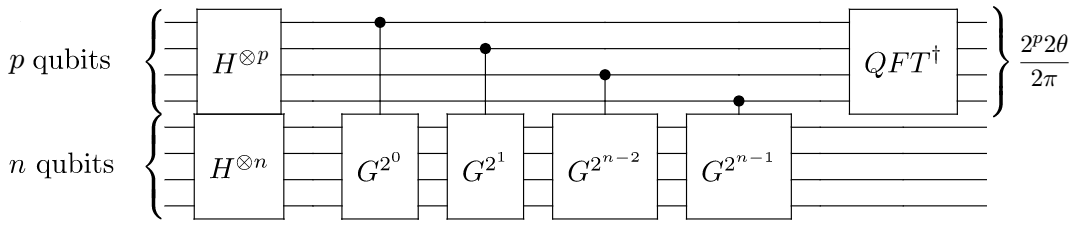
\includegraphics[width=0.9\linewidth]{Figuras/Fig_QC_QPE_G.png}
	\caption{Circuito para la QFE en el caso de Grover.}
	\label{Fig_QC_QPE_G}
	\end{figure}

Como acabamos de comentar, al aplicar QFE mediremos un valor $\tilde{f} = 2^p\tilde{\theta} / \pi$. Podemos despejar $\tilde{\theta}$ y usar (\ref{ec_t-sols_theta}) para calcular $\tilde{M}$
\begin{equation} \label{ec_QC_medidas}
\tilde{\theta} = \frac{\tilde{f} \pi}{2^p} \rqa \tilde{M} = 2^n \, \sin^2 \tilde{\theta} = 2^n \, \sin^2 \frac{\tilde{f} \pi}{2^p},
\end{equation}
donde las $\tilde{\theta}$, $\tilde{f}$ y $\tilde{M}$ llevan una tilde para diferenciarlos de los valores reales. Esto es, porque dependiendo del como de grande sea $p$ (cuantos qubits tengamos en el registro de conteo) nos acercaremos más a medir el valor real del ángulo $\theta$. 

	\begin{mybox}{Nota}
	Como veremos en la sección \ref{sub-sec_U_s}, muchas veces en vez de implementar el operador de 
	difusión $U_{\Psi_0}$ (ver Ec. (\ref{ec_t-sols_Uw_Us})) en realidad se implementa $-U_{\Psi_0}$. 
	En una búsqueda de Grover normal, esta fase es global 
	y no afecta al resultado, pero ahora estamos aplicando versiones controladas del operador de Grover 
	$G$, con lo que esta fase afecta. En esencia, el único cambio es que en realidad estamos contando 
	aquellos estados que \textit{no son solución}. Lo único que tenemos que hacer para obtener el número 
	de soluciones es restar al total de estados, $N$, el valor que obtenemos de aplicar QFE. 
	\end{mybox}

\subsubsection{Precisión de $\tilde{M}$ respecto a $M$.}

Podemos evaluar la precisión del valor de $\tilde{M}$ respecto al valor real $M$, acotando la desviación entre los mismos a medida que variamos $p$. Para ello, vamos a empezar asumiendo que la diferencia entre el valor real y el medido es menor que uno, es decir, $| f- \tilde{f}| <1$. Esto sucede con una probabilidad razonable si $f$ es suficientemente grande (si $p$ es suficientemente grande). Teniendo en cuenta la Ec. (\ref{ec_QC_medidas}), vemos que
\begin{equation*}
| f- \tilde{f}| < 1 \rqa | \theta - \tilde{\theta}| < \frac{\pi}{2^p} \rqa | \sin \theta - \sin \tilde{\theta}| < \frac{\pi}{2^p},
\end{equation*}
donde en la última expresión se ha tenido en cuenta que $\sin \theta \approx \theta$ si $\theta$ es pequeño, lo cual es lógico si consideramos $M << N$. Jugando con las desigualdades puede verse que
\begin{equation} \label{ec_QC_error}
\boxed{|M - \tilde{M}| <   \frac{2 \pi}{2^p} \sqrt{M N} + \frac{\pi^2}{(2^p)^2} N}.
\end{equation}

	\begin{mybox_green}{Derivación de la Ec. (\ref{ec_QC_error})}
	Teniendo en cuenta las desigualdades anteriores, podemos derivar la expresión deseada
	\begin{equation*}
	|M - \tilde{M}|  < N \left| sin^2 \theta - sin^2 \tilde{\theta}  \right|  =   
	N \left| \sin \theta -  \sin \tilde{\theta} \right| 
	\left| \sin \theta + \sin \tilde{\theta} \right|   < 
	N \frac{\pi}{2^p} \lp \sin \theta + \sin \tilde{\theta} \rp.
	\end{equation*}
	En la última igualdad hemos quitado el valor absoluto porque es una suma de dos 
	términos positivos ($0 < \theta < \pi/2$). Precisamente, como estos dos senos son 
	positivos podemos escribir
	\begin{equation*}
	\left| \sin \theta - \sin \tilde{\theta} \right| < \frac{\pi}{2^p} \rqa
	\lch \begin{matrix}
		& \sin \tilde{\theta} <  \sin \theta + \frac{\pi}{2^p} \\
		& \sin \theta <  \sin \tilde{\theta} + \frac{\pi}{2^p} .
	\end{matrix} \right. 
	\end{equation*}
	Esto es porque tenemos dos números positivos que se diferencian en menos de una cierta 
	cantidad $\alpha$, así que es siempre cierto que la suma de uno de los números más 
	$\alpha$ es mayor que el otro. Podemos usar la primera de estas desigualdades para 
	seguir con el cálculo
	\begin{equation}
	|M - \tilde{M}|  < N \frac{\pi}{2^p} \lp \sin \theta + \sin \tilde{\theta}  \rp < 
	N \frac{\pi}{2^p} \lp 2 \sin \theta +\frac{\pi}{2^p} \rp
	\end{equation}
	Finalmente, llegamos a la Ec. (\ref{ec_QC_error})
	\end{mybox_green}

Como podemos ver, la precisión depende de $p$. Además, el tiempo de ejecución depende de $p$, con lo que lo ideal es elegir un valor de $p$ suficientemente grande como para tener una buena precisión, pero que este valor de $p$ no sea demasiado grande y el algoritmo no tarde demasiado. Tomemos $c$ como un parámetro y veamos diferentes casos:
\begin{itemize}
	\item Si tomamos $2^p = c \sqrt{N}$, el error de nuestra estimación de $M$ esta acotado por $\frac{2 \pi}{c} \sqrt{M} + \frac{\pi^2}{c^2}$ siempre que $|f - \tilde{f}| < 1$. Esto recuerda a encontrar la respuesta hasta unas pocas desviaciones estándar. 
	
	\item Si nos conformamos con tener un error \textit{relativo} pequeño, podemos correr el algoritmo para sucesivos valores de $p$ hasta que $\tilde{f}$ sea razonablemente grande. Esto sucederá cuando $2^p = c \sqrt{N/M}$. Después de un tiempo proporcional a $\sqrt{N/M}$, esto nos dará una estimación para $M$ que probablemente estén dentro de un factor $(1+ \pi/c)^2$ de la respuesta correcta. 
	
	\item Si queremos que el error \textit{absoluto} esté probablemente limitado por una constante, aplicamos el algoritmo una vez para $2^p = c \sqrt{N}$ con el objetivo de estimar $M$. Entonces, ejecutamos otra vez, pero esta vez con $2^p = c \sqrt{\tilde{M}N}$. De acuerdo con la Ec. (\ref{ec_QC_error}), pero suponiendo $2^p = c \sqrt{MN}$ por simplicidad, el error resultante en nuestra segunda estimación de $M$ es probable que esté acotado por $\frac{2 \pi}{c} + \frac{\pi^2}{c^2 M}$. En particular, obtenemos una solución exacta, siempre que $|f - \tilde{f}| < 1$, si tomamos $c \geq 14$ ya que $\frac{2 \pi}{c} + \frac{\pi^2}{c^2 M} < \frac{1}{2}$ en ese caso. (Obsérvese que si aplicaciones sucesivamente el algoritmo de Grover y vamos tachamos las soluciones a medida que se encuentran también nos proporcionará un recuento exacto con alta probabilidad en un tiempo en $\mathcal{O} (\sqrt{M N})$, pero con un consumo enorme de memoria. Ver \cite{Approximate_QC}.)
	
	\item Finalmente, comentar que si estamos en el caso en el que el número de soluciones es un cuadrado perfecto pequeño, podemos encontrar el valor  exacto en un tiempo $\mathcal{O}(\sqrt{N})$ con una probabilidad de error muy pequeña. 
	
\end{itemize}

Para más detalles sobre el tema, puede verse \cite{Approximate_QC}.



\newpage
\section{Consideraciones sobre la implementacion} \label{sec_cons_imple}

\subsection{Creación de un difusor $U_{\Psi_0}$.} \label{sub-sec_U_s}

Vamos a ver como podemos hacer para crear de forma genérica un difusor de la forma de (\ref{ec_t-sols_Uw_Us}). Refrescando un poco la memoria, el difusor es un operador realiza una reflexión respecto al estado inicial $| \Psi_0 \rangle$, es decir, \textbf{le cambia el signo a las componentes perpendiculares a} $\bm{| \Psi_0 \rangle}$. Lo que vamos a hacer para construir el difusor es, en realidad, construir un operador que  \textbf{le cambia el signo a las componentes paralelas a} $\bm{| \Psi_0 \rangle}$, es decir, vamos a implementar $-U_{\Psi_0}$. 

Empecemos definiendo la familia de \textbf{operadores de reflexión} $S_A$
\begin{equation} \label{ec_consideraciones_S_a}
\boxed{S_A | i \rangle = 
	\lch
		\begin{matrix}
			& | i \rangle \quad \text{si } i \not \in A \\
			& - | i \rangle \quad \text{si } i \in A
		\end{matrix}
	\right.}
\end{equation}
Es fácil ver que podemos escribir tanto el oráculo como el difusor en función de los operadores $S_A$
\begin{align}
& U_\omega = S_\omega
& \boxed{U_{\Psi_0} = - S_{\Psi_0}}
\end{align}
Nosotros lo que vamos a construir y implementar es $S_{\Psi_0}$, no $U_{\Psi_0}$

\subsubsection{Caso con $N = 2^n$.}

En el caso en el que el estado inicial es una superposición uniforme de la forma (\ref{ec_geo_phi_0_H}) podemos construir el difusor teniendo en cuenta que
\begin{equation}
|\Psi_0 \rangle = H^{\otimes n} |0 \rangle \rqa H^{\otimes n} |\Psi_0 \rangle = |0 \rangle.
\end{equation}
Viendo esta propiedad, podemos darnos cuenta de que si aplicamos el operador de Walsh-Hadamard $H^{\otimes n}$ a la salida del oráculo lo que obtenemos es el estado $| 0 \rangle$ más una serie de estado que corresponderán a los cambios respecto al estado inicial que ha realizado el oráculo. Lo que tenemos que hacer para aplicar el difusor es cambiarle el signo al estado $| 0 \rangle$ (aplicar $S_0$) y volver a aplicar $H^{\otimes n}$ para deshacer los cambios introducidos por la última aplicación el mismo. Es decir, el difusor será de la forma
\begin{equation}
U_{\Psi_0} = - S_{\Psi_0}= - H^{\otimes n} S_0 H^{\otimes n}
\end{equation}
Podemos construir $S_0$ a partir de la \textbf{puerta multicontrolada Z} ($MCZ$)
\begin{equation}
MCZ = 
	\lp
		\begin{matrix}
			& 1 & 0  & \dots & 0 & 0 \\
			& 0 & 1  & \dots & 0 & 0 \\
			& \vdots  & \vdots & \ddots & \vdots & \vdots \\
			& 0 & 0 & \dots & 1 & 0 \\
			& 0 & 0 & \dots & 0 & -1 \\
		\end{matrix}
	\rp
\end{equation}
que lo que hace es cambiarle el signo al estado $|2^n-1\rangle= | 11 \dots 1\rangle$. Tenemos pues
\begin{equation}
S_0 = X^{\otimes n} (MCZ) X^{\otimes n}
\end{equation}
La puerta $X^{\otimes n}$ (que consiste en aplicar puertas $X$ a todos los qubits) lo que hace es 
\begin{align*}
& |00 \dots 0 \rangle \rightarrow |11 \dots 1 \rangle \, \, \Lc |0 \rangle \rightarrow | 2^n-1 \rangle \Rc \\
& |11 \dots 1 \rangle \rightarrow |00 \dots 0 \rangle \, \, \Lc |2^n-1 \rangle \rightarrow | 0 \rangle \Rc
\end{align*}
De esta forma, lo que hace $S_{0}$ es: 
\begin{enumerate}
	\item Aplicar la puerta $X^{\otimes n}$ para cambiar el estado $|00 \dots 0 \rangle$ por el estado $|11 \dots 1 \rangle$. (Ver la Nota de abajo)
	
	\item Aplicar la puerta $MCZ$ con la que cambiamos el signo a $|11 \dots 1 \rangle$ 
	
	\item Aplicar la puerta $X^{\otimes n}$ para deshacer los cambios del primer paso. De esta forma, el único cambio real es el del signo del estado $|0\rangle = |00 \dots 0 \rangle$.
\end{enumerate}

	\begin{mybox}{Nota}
	En realidad la puerta $X^{\otimes n}$ afecta a todos los estados (no solo a $|00 \dots 0 \rangle $ y $|11 \dots 1 \rangle$).
	Sin embargo, como es su propia inversa ($X^{\otimes n}X^{\otimes n} = I$) y como entre la primera y la segunda 
	aplicación de $X^{\otimes n}$ lo único que hacemos 	es cambiarle al signo a $|11 \dots 1 \rangle$, todos los 
	cambios se deshacen menos este signo, que pasa a estar en el estado $|00 \dots 0 \rangle $. 
	\end{mybox}

Como ya comentamos,\textbf{ el operador que se implementa es} $\bm{-U_{\Psi_0}}$, es decir
\begin{align}
& \boxed{-U_{\Psi_0}  = S_{\Psi_0}  = H^{\otimes n} S_0 H^{\otimes n} = H^{\otimes n} X^{\otimes n} (MCZ) X^{\otimes n} H^{\otimes n}} \Rightarrow \label{ec_cons-imple_U_Psi0} \\ 
& \boxed{G_{imple}  =  - U_{\Psi_0} U_\omega = - H^{\otimes n} S_0 H^{\otimes n} U_\omega}
\end{align}



\subsubsection{Caso con $N \neq 2^n$.} \label{sub-sec_N-no-2^n} \label{subsec-N_neq_2n}

Las limitación que hemos impuesto hasta ahora diciendo que $N$ debía ser una potencia de $2$ viene de la transformación de Walsh-Hadammard 
\begin{equation}
H^{\otimes n} |j \rangle = \frac{1}{\sqrt{N}} \sum^{N-1}_{i=0} (-1)^{i \cdot j} | i \rangle, \qquad \text{ (donde } i \cdot j \text{ denota el producto escalar binario)}
\end{equation}
Esta transformación, que se usa para generar el estado inicial y se en el difusor, no está bien definida si no se cumple que $N=2^n$.

Esta condición puede ser relajada si\textbf{ sustituimos la transformación de Walsh-Hadammard por cualquier otra transformación unitario $F$ que cumpla}
\begin{equation} \label{ec_N-no-2n_T}
\boxed{F |0 \rangle = \frac{1}{\sqrt{N}} \sum^{N-1}_{i=0} | i \rangle}
\end{equation}
y seguiremos teniendo interaciones de Grover válidas aplicando 
\begin{equation}
F S_0 F^{-1} U_\omega
\end{equation}
De hecho, cuando estamos en el caso $N = 2^n$, la Walsh-Hadammard es simplemente la elección más sencilla de $F$. Para el caso en el que $N$ no es una potencia de dos, podemos usar la transformación de Fourier de Kitaev \cite{kitaev1995quantum}. Puede verse también \cite{PhysRevLett.80.4329} 

%\textcolor{red}{ESTO LO INTENTÉ MIRAR UN POCO POR ENCIMA Y SE COMPLICA BASTANTE LA COSA.. VALE, ENCONTRÉ UN PAPER INTERESANTE: 4\_Any-Transformation\_PhysRevLett.80.4329}




\newpage
\section{Distribución de probababilidad inicial aleatoria} \label{sec_arbitrary_distribition}

En esta sección vamos a ver una generalización del algoritmo de Grover para el caso en el que partimos de una distribución de probabilidad aleatoria (no uniforme). Veremos como este algoritmo generalizado sigue requiriendo un número de iteraciones $\mathcal{O}(\sqrt{N/M})$, aunque veremos también que hay ciertos casos particularmente desfavorables donde no podemos encontrar ninguna solución. 


Este caso es de especial interés si tenemos en cuenta que muchas veces hay errores al aplicar las puertas. De esta forma, podemos tener errores en el paso de inicialización de la distribución uniforme y acabar con una distribución que se distancia un poco de esta. Como veremos a continuación, el algoritmo de Grover sigue funcionando en presencia de estos errores modestos.

En la siguientes subsecciones presentaremos el algoritmo y derivaremos las ecuaciones diferenciales que rigen la evolución de las amplitudes. Usaremos la solución (exacta) de las mismas para calcular la probabilidad de éxito y analizaremos la diferente casuística. Como el cálculo, aunque simple, puede hacerse pesado, se incluye al final un resumen de con las conclusiones importantes (sección \ref{sec_prop-no-uni_resumen}).

\subsection{Algoritmo}

En realidad, el algoritmo no tiene ningún misterio. Consiste simplemente en saltarse al paso de la inicialización con las puertas de Hadammard y partir del estado con una distribución aleatoria:

\begin{enumerate}
	\item Utilizar cualquier distribución inicial, por ejemplo, el estado final de cualquier otro algoritmo cuántico (no inicializar el sistema con la distribución uniforme).
	
	\item Aplicar el operador de Grover $T$ veces (calcularemos $T$). El operador de Grover al que nos referimos aquí es el mismo de las anteriores secciones (con la Walsh-Hadammard o con una trasformación de la forma (\ref{ec_N-no-2n_T})). No cambia nada en ese sentido.
	
	\item Medir el resultado
\end{enumerate}


\subsection{Evolución de las amplitudes ($M$ soluciones)}

Analicemos la evolución de las amplitudes en el algoritmo modificado. Supongamos (como siempre) que tenemos $N$ estados y $M$ soluciones. Asumamos, sin perdida de generalidad, que $0 \leq M \leq N/2$. El estado total ahora será de la forma
\begin{equation} \label{ec_prob-no-uni_phi-j}
\boxed{|\Psi(t) \rangle = \sum_{i \in \omega} k_i(t) |i \rangle + \sum_{i \in \omega^\perp} l_i(t) |i \rangle }.
\end{equation}
Nótese que ahora las amplitudes tenemos un índices $i$ que corresponde al estado al que acompañan. Esto es fácil de entender: como la distribución de partida ahora no es uniforme, cada estado tendrá su amplitud. Las medias de las amplitudes de los estados solución ($i \in \omega$) y no solución ($i \in \omega^\perp$) son
\begin{align} \label{ec_prop-no-uni_k-l-mean}
& \boxed{\bar{k}(t) = \frac{1}{M} \sum_{i \in \omega} k_i(t) }
& \boxed{\bar{l}(t) = \frac{1}{N-M} \sum_{i \in \omega^\perp} l_i(t)}.
\end{align}
Una de las conclusiones clave del desarrollo que vamos a ver a continuación es que \textit{la dinámica dictada por el algoritmo de Grover se puede describir por completo basándose en la dependencia de las medias de las amplitudes con las iteraciones}.

\subsubsection{Derivación de las ecuaciones diferenciales} \label{subsec_prop-no-uni_ecuaciones-diff}

Comencemos viendo la expresión de la media total de las amplitudes el estado $|\Psi(t) \rangle$
\begin{equation}
\bar{\psi}(t) = \frac{1}{N} \lc \bar{k}(t) + (N-M) \bar{l}(t) \rc,
\end{equation}
y definamos la cantidad $C(t)$
\begin{equation}
C(t) = \frac{2}{N} \lc (N-M) \bar{l}(t) - M \bar{k}(t) \rc.
\end{equation}

Veamos como evolucionan las medias de las amplitudes con cada iteracións:
\begin{itemize}
	\item Después a aplicar el oráculo sobre el esto $|\Psi(t) \rangle$ lo que sucede es el signo de la amplitud de los estados solución se invierte, con lo que 
{
\extrarowheight = -0.5ex
\renewcommand{\arraystretch}{1.75}
\begin{equation*}
\lch \begin{matrix} 
	& \bar{k}(t) \, \rightarrow \, \bar{k^{'}}(t) = -\bar{k}(t) \\
	& \bar{l}(t) \, \rightarrow \, \bar{l^{'}}(t) = \bar{l}(t)
\end{matrix} \right.
\rqa
\overline{U_\omega \psi}(t) = \frac{1}{N} \lc - \bar{k}(t) + (N-M) \bar{l}(t) \rc = \frac{C(t)}{2}.
\end{equation*}
}
	
	\item Después a aplicar el difusor sobre el esto $|\Psi(t) \rangle$ lo que sucede es una reflexión respecto a la media $\overline{U_\omega \psi}(t)$. Esto se pude expresar de la siguiente manera
\begin{align}
{k}^{'}_i(t) \, & \rightarrow \, {k}_i(t) = 2 \overline{U_\omega \psi}(t) - {k}^{'}_i(t) =  C(t) - k^{'}_i(t) = C(t) + k_i(t) \label{ec_prop-no-uni_k-j+1_i} \\
{l}^{'}_i(t) \, & \rightarrow \, {l}_i(t) = 2 \overline{U_\omega \psi}(t) - {l}^{'}_i(t) = C(t) - l^{'}_i(t) C(t) - l_i(t). \label{ec_prop-no-uni_l-j+1_i} 
\end{align}
Promediando
\begin{align}
\Aboxed{\bar{k}(t+1) = C_j + \bar{k}(t) } \label{ec_prop-no-uni_k-j+1} \\
\Aboxed{\bar{l}(t+1) = C_j - \bar{l}(t)}.  \label{ec_prop-no-uni_l-j+1} 
\end{align}
\end{itemize}
Las Ecs. (\ref{ec_prop-no-uni_k-j+1}) y (\ref{ec_prop-no-uni_l-j+1}) son las ecuaciones diferenciales que rigen la evolución de la media de las amplitudes.


\subsubsection{Soluciones de las ecuaciones diferenciales} \label{subsec_prop-no-uni_ecuaciones-diff-sol}

Vamos a resolver de forma analítica las Ecs. (\ref{ec_prop-no-uni_k-j+1}) y (\ref{ec_prop-no-uni_l-j+1})  para ver la evolución exacta de las medias de las amplitudes de los estados solución y no solución. Procedemos a resolver las fórmulas de recursión para condiciones iniciales complejas arbitrarias. Empecemos definiendo las funciones
\begin{align}
\Aboxed{& f_{+}(t) = \bar{l}(t) + i \sqrt{\frac{M}{N-M}} \bar{k}(t)} \label{ec_prop-no-uni_f+}\\
\Aboxed{& f_{-}(t) = \bar{l}(t) - i \sqrt{\frac{M}{N-M}} \bar{k}(t)}. \label{ec_prop-no-uni_f-}
\end{align}
Vemos que no son más que un \textbf{cambio de variables} para facilitarnos la resolución de las ecuaciones. Empleando este cambio de variables podemos reescribir las Ecs. (\ref{ec_prop-no-uni_k-j+1}) y (\ref{ec_prop-no-uni_l-j+1}) de la siguiente forma
\begin{align}
& f_{+}(t+1) = e^{i \beta} f_{+}(t) \\
& f_{-}(t+1) = e^{- i \beta} f_{-}(t),
\end{align}
donde $\beta$ es \textbf{real} y cumple
\begin{equation} \label{ec_prop-no-ini_beta}
\boxed{\cos \beta = 1 - 2 \frac{M}{N}}.
\end{equation}
Vemos que ahora la solución de las ecuaciones es trivial:
\begin{align}
& f_{+}(t) = e^{i \beta t} f_{+}(0) \\
& f_{-}(t) = e^{-i \beta t} f_{-}(0).
\end{align}
Vemos claramente que $| f_{+}(t) |$ y $|f_{-}(t)|$ son independientes de la iteración $t$ en la que estemos. Podemos ahora deshacer el cambio de variable 
\begin{align}
\Aboxed{\bar{k}(t) & = - i \sqrt{\frac{N-M}{4M}} \lc e^{i \beta t} f_{+}(0) - e^{-i \beta t} f_{-}(0)  \rc}  \label{ec_prop-no-uni_sol_k} \\
\Aboxed{\bar{l}(t) & = \frac{1}{2} \lc e^{i \beta t} f_{+}(0) - e^{-i \beta t} f_{-}(0)  \rc }.  \label{ec_prop-no-uni_sol_l}
\end{align}


\subsection{Propiedades de las soluciones: Probabilidad de acierto.}


\subsubsection{Evolución de las amplitudes en función de la evolución de las medias.} 

Lo primero que vamos a hacer es ver que, efectivamente, solo con la evolución de las medias podemos describir la evolución. 
Para ello, restemos a la Ec. (\ref{ec_prop-no-uni_k-j+1_i}) la Ec. (\ref{ec_prop-no-uni_k-j+1}) y a la Ec. (\ref{ec_prop-no-uni_k-j+1_i}) restémosle la Ec. (\ref{ec_prop-no-uni_k-j+1})
\begin{align*}
k_i(t+1) - \bar{k}(t+1) & = k_i(t) - \bar{k}(t) \\
l_i(t+1) - \bar{l}(t+1) & = - \lc l_i(t) - \bar{l}(t) \rc.
\end{align*}
Esto significa que las cantidades
\begin{align}
\Delta k_i & \equiv k_i(0) - \bar{k}(0) \\
\Delta l_i & \equiv l_i(0) - \bar{l}(0) 
\end{align}
son \textit{constantes del movimiento}. Esto nos permite simplificar las expresiones para la dependencia temporal de las amplitudes:
\begin{align}
\Aboxed{k_i(t) & = \bar{k}(t) + \Delta k_i} \label{ec_prop-no-uni_k-delta}\\
\Aboxed{l_i(t) & = \bar{l}(t) + (-1)^t \Delta l_i}. \label{ec_prop-no-uni_l-delta}
\end{align}
Vemos que  la distribución de las amplitudes de los estados solución $k_i(t)$ respecto a su medias $\bar{k}(t)$ es constante. Es decir, las amplitudes varían al unísono entorno a la medias. De esta forma, con saber las distribución inicial respecto a las medía ($\Delta k_i$) podemos describir la evolución de las amplitudes solo conociendo la evolución de las medias. Lo mismo sucede para los estados no solución $l_i(t)$, salvo que estos se invierten entorno a su media en cada iteración.

De las Ecs. (\ref{ec_prop-no-uni_k-delta}) y (\ref{ec_prop-no-uni_l-delta}) se ve inmediatamente que las varianzas
\begin{align*}
\sigma_k^2 (t) & = \frac{1}{M} \sum_{i \in \omega} |k_i(t) - \bar{k}(t)|^2   \\
\sigma_l^2 (t) & = \frac{1}{N-M} \sum_{i \in \omega^\perp} |l_i(t) - \bar{l}(t)|^2 
\end{align*}
son independientes del tiempo [$\sigma_k^2 (t) = \sigma_k^2 (0)$ y $\sigma_l^2 (t)=\sigma_l^2 (0)$ $ \forall t$].



\subsubsection{Probabilidad de acierto.} \label{subsec_prop-no-uni_Pt}

Para facilitar el análisis de las soluciones, definamos las variables (complejas) $\alpha$ y $\phi$ de la forma
\begin{align} \label{ec_prop-no-uni_alpha_phi}
& \alpha = \sqrt{f_{+}(0) f_{-}(0)},
& e^{2i\phi} = f_{+}(0)/f_{-}(0).
\end{align}
Reescribamos las Ecs. (\ref{ec_prop-no-uni_sol_k}) y (\ref{ec_prop-no-uni_sol_l}) en función de estas variables
\begin{align}
\Aboxed{\bar{k}(t) & = \sqrt{\frac{N-M}{M}} \alpha \sin ( \beta t + \phi)}  \label{ec_prop-no-uni_sol_k-2} \\
\Aboxed{\bar{l}(t) & = \alpha \cos (\beta t + \phi)} \label{ec_prop-no-uni_sol_l-2}
\end{align}
Esto nos permite ver que hay una diferencia de fase de $\pi/2$ entre las medias de las amplitudes de los estados solución y los no solución. Se ve fácilmente que cuando una es máxima, la otra es mínima. 

La probabilidad de medir alguno de los estados solución será $P(t) = \sum_{i \in \omega} |k_i(t)|^2$. Como todos los operadores son unitarios, las amplitudes cumplen la condición de normalización:
\begin{equation} \label{ec_prop-no-uni_unitaridad}
\sum_{i \in \omega} |k_i(t)|^2 + \sum_{i \in \omega^\perp} |l_i(t)|^2 = 1 \quad \forall t
\end{equation}
Usando la identidad
\begin{equation} 
\overline{(y-\bar{y})^2} = \overline{y^2} - \bar{y}^2 \rqa \sigma_y^2 = \overline{y^2} - \bar{y}^2 
\rqa  \overline{y^2} = \sigma_y^2  + \bar{y}^2  
\end{equation}
podemos escribir
\begin{align*}
\overline{|k_i(t)|^2} = \frac{1}{M} \sum_{i \in \omega} |k_i (t) |^2 = \sigma_k^2 + |\bar{k}(t)|^2 \\
\overline{|l_i(t)|^2} = \frac{1}{N-M} \sum_{i \in \omega} |l_i (t) |^2 = \sigma_l^2 + |\bar{l}(t)|^2 
\end{align*}
Despejando $\sum_{i \in \omega} |k_i(t)|^2$ en (\ref{ec_prop-no-uni_unitaridad}), sustituyendo en $P(t)$, usando la expresión anterior de $\sum_{i \in \omega} |l_i (t) |^2 $ y desarrollando con cuidado, puede verse que %\textcolor{red}{(Horroroso desarrollo. Yo no fuí capaz de sacarlo. Para mi el $\text{Re}(\phi)$ es magia potagia. Simplemente creo que sigue los pasos que dije en este parágrafo pero ni seguro estoy.)}
\begin{equation} \label{ec_prop-no-uni_Pt}
\boxed{P(t) = P_{av} - \Delta P \cos 2\lc \beta t + \text{Re}(\phi) \rc ,}
\end{equation}
donde 
\begin{align*}
& P_{av} = 1- (N-M) \sigma_l^2 - \frac{1}{2} \Lc (N-r) |\bar{l}(0)|^2 + r |\bar{k}(0)|^2 \Rc \\
& \Delta P = \frac{1}{2} \Bigl| (N-M) \bar{l}(0)^2 + M \bar{k}(0)^2 \Bigr|
\end{align*}

\subsubsection{Número optimo, $T$, de iteraciones.} \label{subsec_prop-no-uni_T}

El valor máximo de la probabilidad que se puede obtener durante la evolución del algoritmo es
\begin{equation}
P_{max}=P_{av} + \Delta P
\end{equation}
Dada una distribución arbitraria inicial de $M$ estados solución y $N-M$ estados no solución, con medias $\bar{k}(0)$ y $\bar{l}(0)$ respectivamente, el valor máximo de la probabilidad $P_{max}$ se alcanzará cuando realicemos $T$ iteraciones tal que
\begin{equation} \label{ec_prop-no-uni_T}
\cos 2 \lc \beta T + \text{Re} (\phi) \rc =1 \rqa 
\boxed{T = \lc (u + 1/2)  \pi - \text{Re} (\phi) \rc/\beta}
\end{equation}
con $u = 0,1,2,\dots$. Una importante conclusión es que para determinar el valor óptimo de iteraciones, todo lo que necesitamos es conocer \textit{las medias iniciales de las amplitudes y el número de estados marcados}.

Si $M$ es pequeño tenemos que $1-2M/N \approx 1$, así que podemos aproximar $\beta$ a primer orden en la Ec. (\ref{ec_prop-no-ini_beta})
\begin{equation}
\cos \beta \approx 1 - \frac{1}{2} \beta^2 = 1- 2 \frac{M}{N} \rqa \beta = 2 \sqrt{\frac{M}{N}}
\end{equation}
Así que tenemos que $T$ es del orden de $\mathcal{O}(\sqrt{N/M})$ (para $u=0$).

\subsubsection{Casos particulares.} \label{subsec_prop-no-uni_casos-particulares}

El valor máximo de la probabilidad puede variar mucho dependiendo de las propiedades estáticas (medias y varianzas) de las distribución inicial de amplitudes. Como es lógico, cuanto mayor sea $P_{max}$ menos repeticiones del algoritmo tendremos que hacer para encontrar una solución (donde cada repetición son $m$ iteraciones). Es fácil darse cuenta de que el número esperado de repeticiones del algoritmo hasta encontrar un estado solución es $1/P_{max}$.

\begin{mybox}{Nota}
Porque \textit{repeticiones del algoritmo}?. En el parágrafo anterior llamamos repeticiones del algoritmo a realizar varias veces las $m$ iteraciones necesarias para maximizar la probabilidad. 

Si la probabilidad máxima es menor de uno, tenemos entonces la posibilidad de tras realizar las $m$ iteraciones no midamos un estado solución. Si esto sucede, como al medir se destruye el estado, lo que hay que hacer es volver a empezar: volver a partir de la distribución inicial y aplicar $m$ iteraciones. En promedio, tendremos que repetir este proceso $1/P_{max}$ veces. Vemos que si la probabilidad máxima es, por ejemplo, $1/4$, tendremos que medir en promedio 4 veces para obtener un estado solución. 
\end{mybox}

Veamos los diferentes casos:
\begin{itemize}
	\item Cuando el ratio $\bar{l}(0)/\bar{k}(0)$ es real, puede verse fácilmente que $|f_+(0)| =f_{-}(0)|$. En este caso $P_{max} = 1-(N-r)\sigma_l^2$. El mejor caso, aquel con $P_{max}=1$, se obtiene cuando $\sigma_l=0$, es decir, cuando la distribución inicial es uniforme.
	
	\item Cuando tenemos $f_+(0)=0$ o $f_-(0)=0$, el algoritmo es inútil, pues $P(t)$ es constante.
	
	\item El peor caso se da cuando $\sigma_k^2=f_+(0)=f_-(0)=\bar{k} (0)=\bar{l}(0)=0$ y $(N-r)\sigma_l^2=1$. En este caso tenemos $P_{max}=P(t)=0$ $\forall t$, con lo que nunca encontraremos una solución.
	
\end{itemize}

\subsubsection{Distribución de probabilidad desconocida.} \label{subsec_prop-no-uni_desconocida}

Veamos que sucede si no conocemos de antemano las medias y las varianzas de la distribución inicial de amplitudes. 
%De las Ec. (\ref{ec_prop-no-ini_beta}) y (\ref{ec_prop-no-uni_Pt}) se ve que el periodo de oscilación de la probabilidad $P(t)$ depende solo de $M/N$, mientras que los detalles de la distribución inicial de amplitudes están en la fase $\phi$. 
La solución es más sencilla de lo que podríamos pensar en un principio. Lo único que hay que hacer es ejecutar el algoritmo dos veces, ejecutando en un caso $m_1$ iteraciones y en el otro $m_2$ iteraciones, tal que $m_2-m_1=\pi/(2 \beta)$. De la Ec. (\ref{ec_prop-no-uni_Pt}) está claro que al menos en uno de los dos caso vamos a tener $P(t)\geq P_{av} \geq P_{max}/2$. En este caso, necesitamos el doble de repeticiones para obtener al menos la mitad de probabilidades de éxito que cuando se conoce el tiempo de medición óptimo. Vemos además que lo único que necesitamos conocer en este caso es $\beta$, que según la Ec. (\ref{ec_prop-no-ini_beta}) podemos calcularlo a partir del número de soluciones $M$.


\subsection{Resumen de la sección.}  \label{sec_prop-no-uni_resumen}

Uno de los puntos importantes del análisis de esta sección es el hecho de demostrar que el algoritmo de Grover funciona incluso en el caso en el que tenemos pequeños errores a la hora de generar la distribución de probabilidad inicial. En realidad, en esta sección no se presenta ningún algoritmo nuevo. Simplemente se analiza que pasa si usamos el algoritmo de Grover donde en el primer paso sustituimos la inicialización de la distribución uniforme por una distribución no uniforme.

Otra de las conclusiones clave del desarrollo es que la dinámica dictada por el algoritmo de Grover se puede describir por completo basándose en la dependencia de las medias de las amplitudes $\bar{k}(t)$ y $\bar{l}(t)$ (definidas en la Ec. (\ref{ec_prop-no-uni_k-l-mean})).

Para estudiar la dependencia con las iteraciones de las medias $\bar{k}(t)$ y $\bar{l}(t)$, en la sección \ref{subsec_prop-no-uni_ecuaciones-diff} deducimos las ecuaciones diferenciales que rigen su evolución (Ecs. (\ref{ec_prop-no-uni_k-j+1}) y (\ref{ec_prop-no-uni_l-j+1})). En la sección \ref{subsec_prop-no-uni_ecuaciones-diff-sol} las resolvemos. Para ello primero hacemos un cambio de variable de $\bar{k}(t)$ y $\bar{l}(t)$ a $f_+(t)$ y $f_-(t)$ (Ecs. (\ref{ec_prop-no-uni_f+}) y (\ref{ec_prop-no-uni_f-})).  Resolvemos usando estas variables y deshacemos el cambio. Nos quedan pues $\bar{k}(t)$ y $\bar{l}(t)$ en función de $f_+(0)$, $f_-(0)$ y $\beta$ (definido $\beta$ en la Ec. (\ref{ec_prop-no-ini_beta}), que solo depende de $N$ y $M$). 

Una vez tenemos las soluciones, en las Ecs. (\ref{ec_prop-no-uni_k-delta}) y (\ref{ec_prop-no-uni_l-delta}) demostramos que las amplitudes mantienen su distribución respecto a las medias invariante (con una salvedad en $\bar{l}(t)$). De esta forma, confirmamos que solo tenemos que conocer la distribución inicial respecto a las medias para describir la evolución de las amplitudes usando solo la evolución de las medias. 

En la sección \ref{subsec_prop-no-uni_Pt}  definimos dos parámetros más, $\alpha$ y $\phi$ (Ec. (\ref{ec_prop-no-uni_alpha_phi})), que depende de $f_+(0)$ y $f_-(0)$. Tras unas líneas de cálculo podemos llegar a la Ec. (\ref{ec_prop-no-uni_Pt}) que nos da la probabilidad $P(t)$ de medir un estado solución en función del número de iteraciones. Una vez tenemos esta expresión, en la sección \ref{subsec_prop-no-uni_T} buscamos el número $T$ de iteraciones que nos maximizan la probabilidad (Ec. (\ref{ec_prop-no-uni_T})). Una importante conclusión es que para determinar el valor óptimo de iteraciones, todo lo que necesitamos es conocer las medias iniciales de las amplitudes y el número de estados marcados. Concluimos también que si $M$ es pequeño, tenemos que $T$ es del orden de $\mathcal{O}(\sqrt{N/M})$.

Finalmente, analizamos casos particulares de distribuciones iniciales favorables y desfavorables (sección \ref{subsec_prop-no-uni_casos-particulares}) y vemos que pasa si no conocemos las distribución de probabilidad inicial (sección \ref{subsec_prop-no-uni_desconocida}). Es este último caso, 
nuevamente podemos hallar una solución en tiempo $\mathcal{O}(N/M)$ conociendo solo $M$. 








\newpage
\section{Implementaciones con qiskit.}

\subsubsection{Puerta multicontrolada $Z$ (MCZ).}

Vamos a empezar viendo la implementación de la puerta multicontrolada $Z$ (MCZ) en qiskit, pues la usaremos bastante el las siguientes secciones. Esta puerta podemos construir a partir de la puerta multicontrolada Toffoli (MCT) de forma muy sencilla. Para ello, recordemos que la MCT no es más que una CNOT (es decir, una puerta $X$) con varios controles y recordemos también la propiedad
\begin{equation} \label{Imple_HXH_Z}
HXH = Z .
\end{equation}
Podemos pues construir la MCZ aplicando puertas de Hadammard en el qubit objetivo de la MCT antes y después de la misma. En código de qiskit esto nos queda 

\begin{lstlisting}
def mcz(circuit, control_qubits, target_qubit):

	circuit.h(target_qubit)
	circuit.mct(control_qubits, target_qubit)  # multi-controlled-toffoli
	circuit.h(target_qubit)

\end{lstlisting}

	\begin{mybox}{Nota}
	Esta función (con su documentación) puede encontrarse también en la carpeta \textit{Code} en el script
	\textit{Grover\_Gates\_and\_functions.py}.
	\end{mybox}


\subsection{Difusor genérico.}

Como ya comentamos en la sección \ref{sub-sec_U_s}, habitualmente en vez de implementar $U_{\Psi_0}$ implementamos $-U_{\Psi_0}$. Vimos además que podemos hacer la implementación mediante transformadas de Walsh-Hadamard $H^{\otimes n}$, puertas $X^{\otimes n}$ y la puerta $MCZ$ de la forma de la Ec. (\ref{ec_cons-imple_U_Psi0}), es decir
\begin{equation} \label{ec_qiskit_diff-gen_U_Psi0}
\boxed{-U_{\Psi_0}  = S_{\Psi_0}  = H^{\otimes n} S_0 H^{\otimes n} = H^{\otimes n} X^{\otimes n} (MCZ) X^{\otimes n} H^{\otimes n}} 
\end{equation} 

Veamos como traducir la Ec. (\ref{ec_qiskit_diff-gen_U_Psi0}) a código qiskit. 
\begin{lstlisting}
def Grover_Diffuser(circuit, target_reg):
	
	n = target_reg.size

	# Apply transformation |s> -> |00..0> (H-gates)
	for i in range(n):
		circuit.h(target_reg[i])

	# Apply transformation |00..0> -> |11..1> (X-gates)
	for i in range(n):
		circuit.x(target_reg[i])

	# Do multi-controlled-Z gate
	mcz(circuit, target_reg[list(range(n-1))], target_reg[n-1])

	# Apply transformation |11..1> -> |00..0>
	for i in range(n):
		circuit.x(target_reg[i])

	# Apply transformation |00..0> -> |s>
	for i in range(n):
		circuit.h(target_reg[i])

\end{lstlisting}


La función anterior es genérica: dado un circuito y un registro cuántico, esta función aplica un difusor de Grover en el registro. En la Fig. \ref{Fig_Imple_diffuser} el resultado de aplicar la función anterior sobre un circuito.


	\begin{figure}[H]
	\centering 
	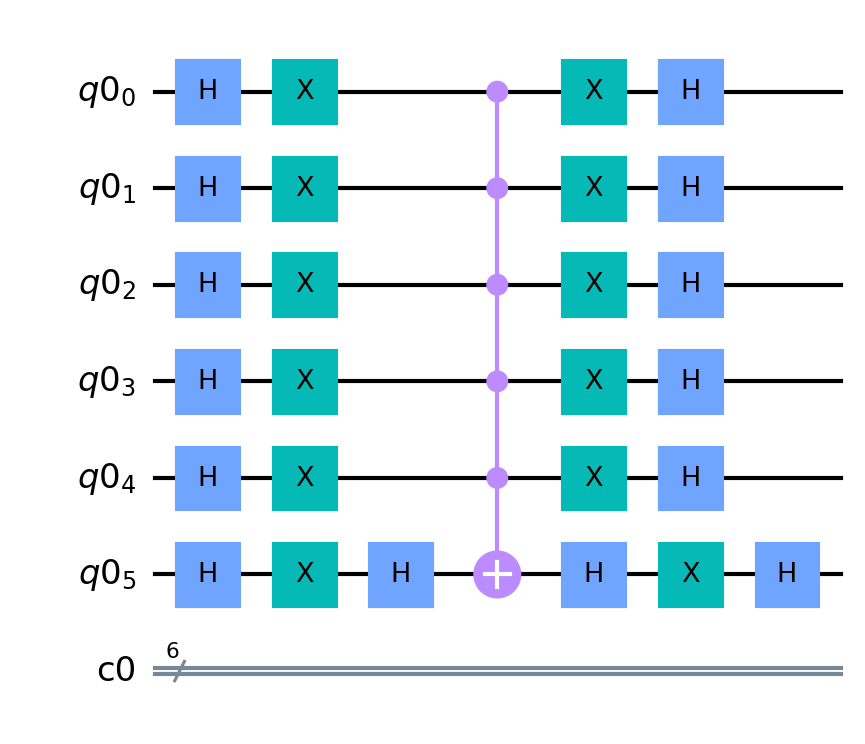
\includegraphics[width=0.5\linewidth]{../Code/Fig_Imple_diffuser.png}
	\caption{Difusor de Grover construido con Qiskit. Código en Grover's\_algoritm$\backslash$Code$\backslash$Grover\_Diffusers.py}
	\label{Fig_Imple_diffuser}
	\end{figure}

	\begin{mybox}{Nota}
	Esta función (con su documentación) puede encontrarse también en la carpeta 
	\textbf{Grover's\_algoritm$\backslash$Code.} (en mismo nivel que la carpeta Theory) en el script  \textbf{Grover\_Diffusers.py}. 
	El script puede usarse como módulo para importar el difusor o simplemente ejecutarse para generar la gráfica. 
	\end{mybox}


\subsection{Oráculo ``trivial''.}

\begin{mybox_red}{Nota Importante!!}
Puede verse una implementación más general y avanzada del oráculo que se va a construir en esta sección en el script \textbf{1-Grover\_trivial\_oracle.py} situado en la carpeta \textbf{Grover's\_algoritm$\backslash$Code.} (en mismo nivel que la carpeta Theory).
\end{mybox_red}

Vamos a presentar en esta sección un código de qiskit para construir un oráculo que cambie el signo de los estados que nosotros le digamos. Este es uno de esos ejemplo típicos que se plantean cuando se habla de Grover, esos en los que sabemos con antelación los estados concretos que queremos buscar. De esta forma, el oráculo que construimos está echo ``ad hoc'' para marcar ciertos estado. Precisamente elegi llamarle a esta caso ``trivial'' porque no entraña ningún misterio, sino que como comento es un caso académico. 


El código que se presenta a continuación es muy simple. Partimos de una lista de cadenas binarias de n bits que llamamos \textbf{M\_list\_bin\_qiskit}. Por ejemplo, para $n=5$
$$
\text{M\_list\_bin\_qiskit} = [\text{'} 01101 \text{'}, \text{'} 11000 \text{'}, ...]
$$

	\begin{mybox}{Nota}
	Recordemos que en qiskit el bit menos significativo es que va arriaba en el circuito, así que 
	el ``qiskit'' en el nombre de la lista \textbf{M\_list\_bin\_qiskit} hace referencia que estamos 
	mandando las cadenas el revés. Es decir, para pasarlas a decimal las invertimos:
	$$
	01101 \quad \rightarrow \quad 10110 = 22, \qquad
	11000 \quad \rightarrow \quad 00011 = 3
	$$
	\end{mybox}


Para cambiar el signo de un estado lo que tenemos que hacer es aplicar una MCZ. Como esta solo aplica sobre el estado $|11\dots 1 \rangle$, lo que hay que hacer es aplicar puertas $X$ antes y después del la MCZ en los qubit correspondientes a las posiciones donde tenemos un 0 en las cadenas bits.

\begin{lstlisting}
def Grover_Oracle_trivial(circuit, target_reg, M_list_bin_qiskit): 

	n = target_reg.size

	circuit.barrier()
	for m in M_list_bin_qiskit:
		for i in range(len(m)):
			if m[i] == '0':
				circuit.x(target_reg[i])

		mcz(circuit, target_reg[list(range(n-1))], target_reg[n-1])
	    
		for i in range(len(m)):
			if m[i] == '0':
				circuit.x(target_reg[i])

\end{lstlisting}

En la Fig. \ref{Fig_Imple_oracle_trivial} podemos ver el resultado de aplicar la función anterior sobre un circuito. 

	\begin{figure}[H]
	\centering 
	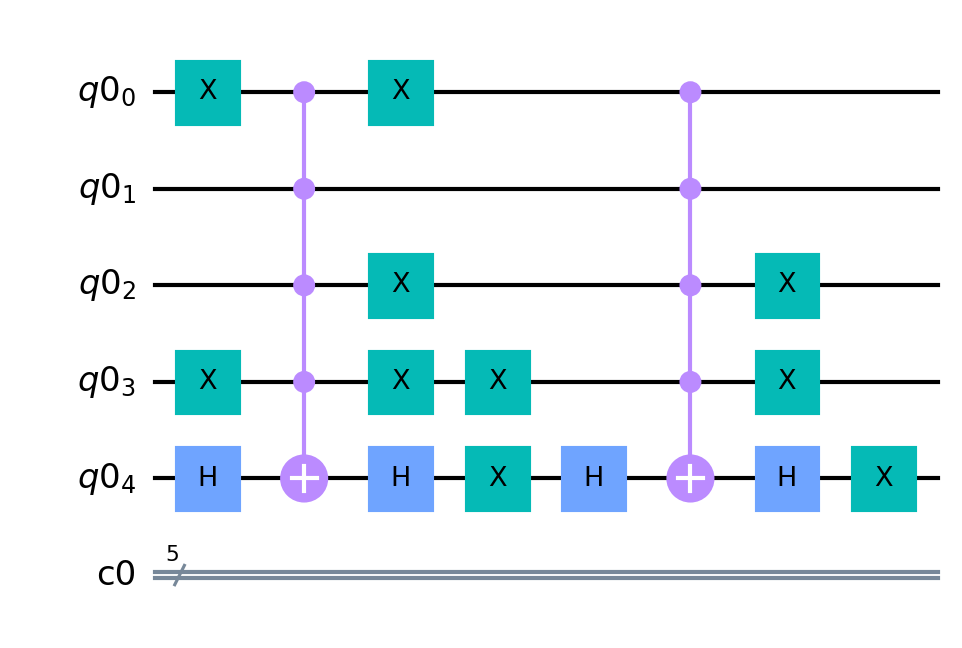
\includegraphics[width=0.6\linewidth]{Theory_Notes_Codes/Fig_Imple_oracle_trivial.png}
	\caption{Oráculo trivial, es decir, para el caso en el que conocemos las soluciones de antemano.  Código en Theory\_Notes\_Codes$\backslash$Oracle\_Trivial.py}
	\label{Fig_Imple_oracle_trivial}
	\end{figure}

	\begin{mybox}{Nota}
	Esta función (con su documentación) puede encontrarse también en la carpeta
	\textbf{Grover's\_algoritm$\backslash$Code.} en el script  \textbf{Grover\_Oracles.py}. 
	 
 	Además, el código que generó la Fig. \ref{Fig_Imple_oracle_trivial} puede encontrarse en el script 
	\textit{Oracle\_Trivial.py} en la carpeta \textit{Theory\_Notes\_Codes}. En este script se un \textit{import}
	del oráculo que está en el script anterior.
	\end{mybox}


\subsection{Oráculos que verifican condiciones.}

En esta sección vamos a ver como se puede usar el algoritmo de Grover para buscar cadenas de bits que satisfacen unas ciertas condiciones. En concreto vamos a ver dos caso: como solucionar un \textbf{sudoku 2x2} y como calcular todas las posibles permutaciones de $P$ números.

\begin{mybox_red}{Nota Importante!!}
Puede verse una implementación más general y avanzada del caso de las permutaciones situado en la carpeta \textbf{Grover's\_algoritm$\backslash$Code.} (en mismo nivel que la carpeta Theory). En esta implementación se usa la idea de buscar números diferentes para calcular las permutaciones de $P$ números. Esta implementación es la ``joya de la corona'' de la explicación que se está dando sobre el algoritmo de Grover.
\end{mybox_red}

\subsubsection{Sudoku 2x2. }

			\subsubii \textit{El sudoku.} 

Vamos a ver en esta sección como construir un oráculo que resuelva un sudoku 2x2 de la forma:
\begin{equation}
	\lc
	\begin{matrix}
	V_0 & V_1 \\
	V_2 & V_3
	\end{matrix}
	\rc
\end{equation}

			\subsubii \textit{Condiciones y puerta XOR.}
			 
En un sudoku tiene que cumplirse que no se repitan números en las filas ni en las columnas, así que las condiciones que tienen que verificar las variables de sudoku 2x2 son:
\begin{equation}
V_0 \neq V_1, \qquad 
V_0 \neq V_2, \qquad
V_2 \neq V_3, \qquad
V_1 \neq V_3.
\end{equation}

Por comodidad, podemos compilar este conjunto de comparaciones en una lista de cláusulas:
\begin{lstlisting}
clause_list = [ [0,1],  [0,2],  [1,3],  [2,3] ]
\end{lstlisting}
Para verificar estas condiciones podemos usar un qubit ancilla y usar la puerta XOR (se puede ver el código a continuación). Como el qubit ancilla parte del estado $|0\rangle$, esta puerta lo que hace ponerlo a en el estado $|1\rangle$ si la condición se verifica.

\begin{lstlisting}
def XOR_2qubits(qc, a, b, output):
    qc.cx(a, output)
    qc.cx(b, output)
\end{lstlisting}

	\begin{figure}[H]
	\centering 
	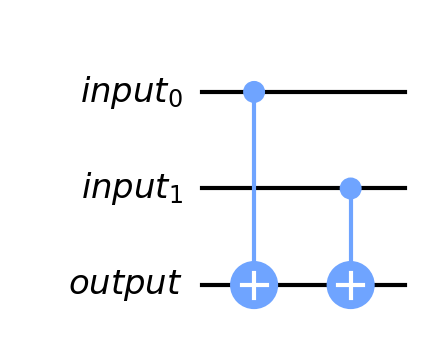
\includegraphics[width=0.25\linewidth]{Theory_Notes_Codes/Fig_Imple_xor.png}
	\caption{Puerta XOR. Código en Theory\_Notes\_Codes$\backslash$XOR.py}
	\label{Fig_Imple_xor}
	\end{figure}

	\begin{mybox}{Nota}
	Esta función (con su documentación) puede encontrarse también en la carpeta 
	\textbf{Grover's\_algoritm$\backslash$Code.} en el script  \textbf{Grover\_Gates\_and\_functions.py}. 
	
	Además, el código que generó la Fig. \ref{Fig_Imple_xor} puede encontrarse en el script
	 \textbf{XOR.py} en la carpeta \textbf{Theory\_Notes\_Codes}. En este script se un \textit{import}
	de la puerta que está en el script anterior.
	\end{mybox}

			\subsubii \textit{Oráculo.} 

Para generar el oráculo del sudoku podemos usar 4 qubits ancila (uno por condición a verificar) y usar la puerta XOR 4 veces. Pero con esto aún no tenemos el oráculo, pues nos falta verificar si todas las condiciones se cumplen y cambiar el signo del estado. Para ello, podemos usar una puerta MCT que tenga como controles los 4 cubits ancilla y que se aplique sobre un quinto qubit que esté en el estado $|-\rangle$. De esta forma, la puerta MCT solo se aplicará si se cumplen las 4 condiciones. Por último, solo nos faltaría volver a aplicar las puertas XOR para limpiar los qubits ancilla. El resultado final sería el siguiente:

\begin{lstlisting}
def sudoku_oracle(circuit, clause_list, clause_qubits):
    # Compute clauses
    i = 0
    for clause in clause_list:
        XOR(circuit, clause[0], clause[1], clause_qubits[i])
        i += 1

    # Flip 'output' bit if all clauses are satisfied
    qc.mct(clause_qubits, output_qubit)

    # Uncompute clauses to reset clause-checking bits to 0
    i = 0
    for clause in clause_list:
        XOR(circuit, clause[0], clause[1], clause_qubits[i])
        i += 1
\end{lstlisting}

	\begin{figure}[H]
	\centering 
	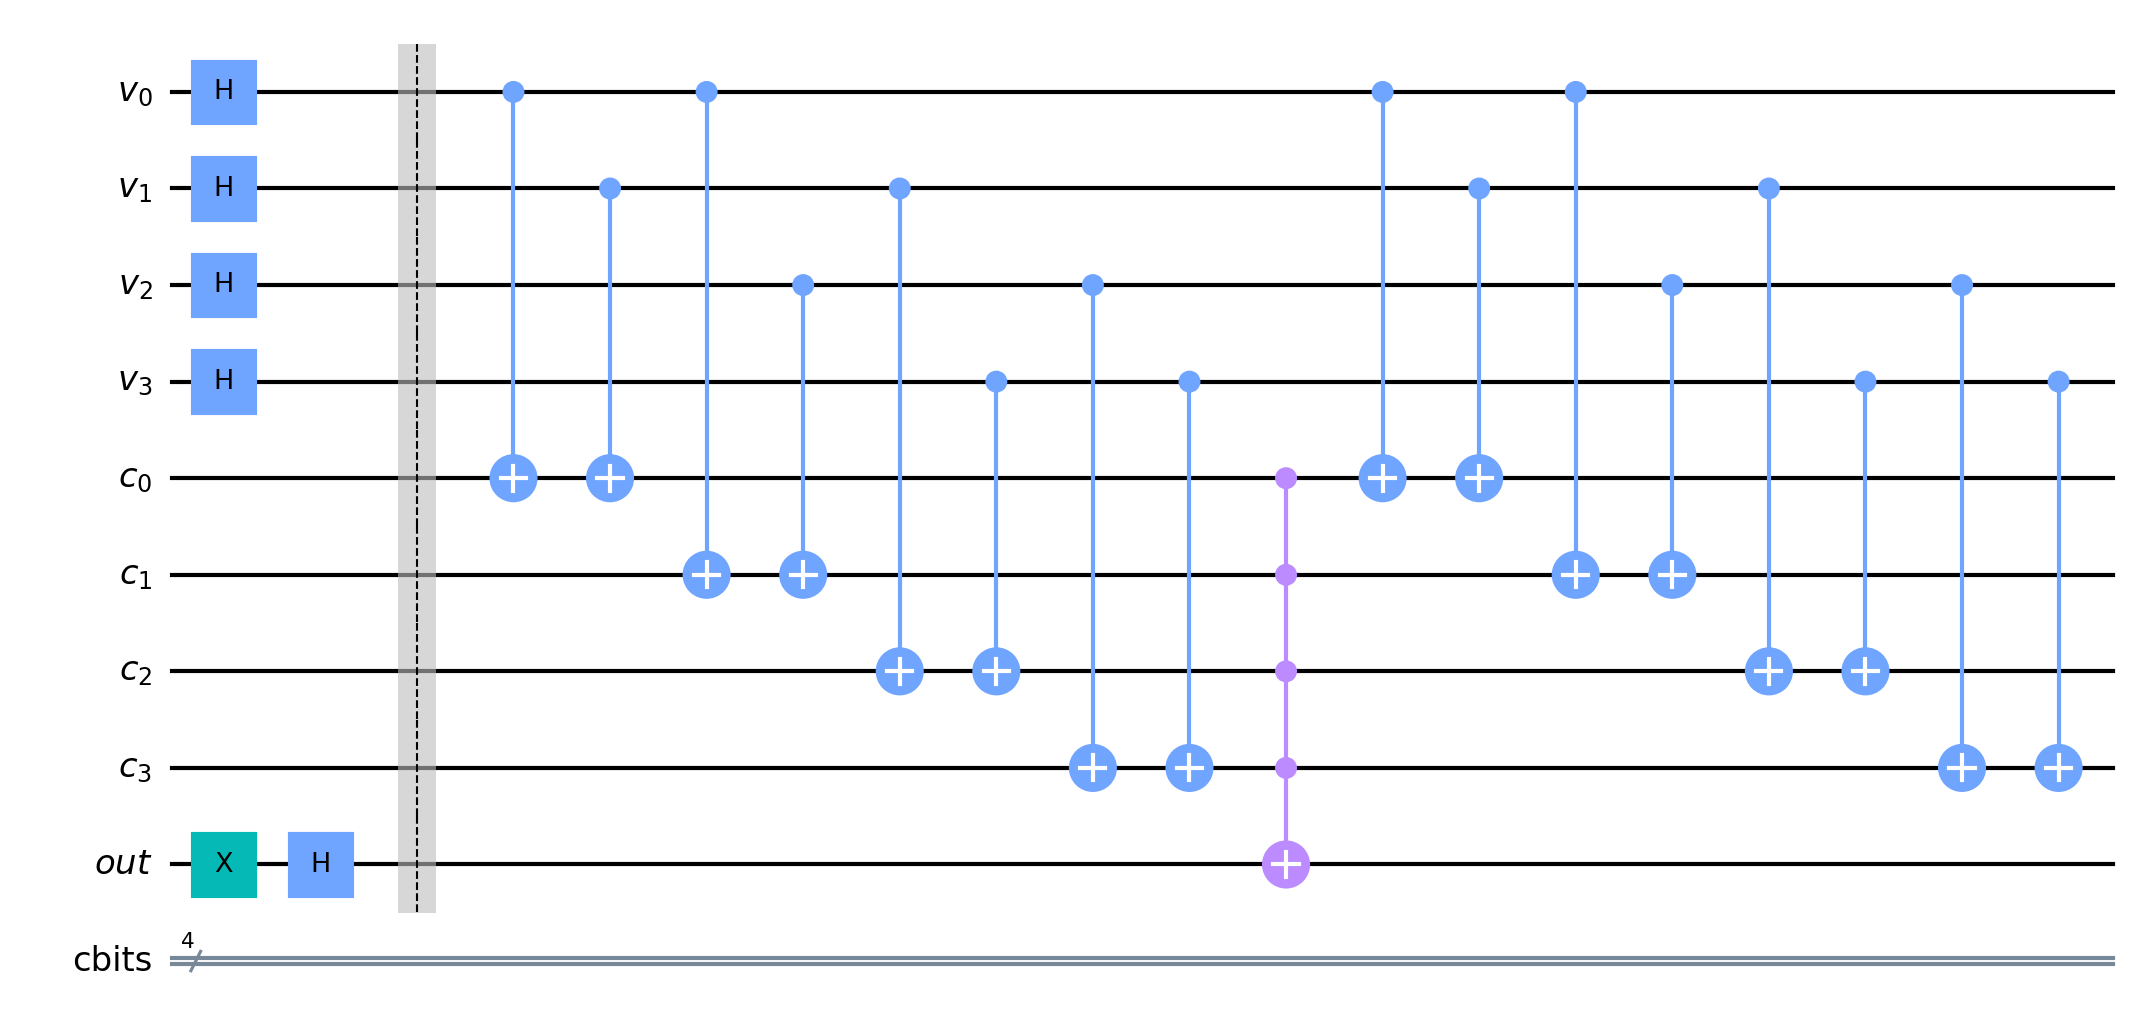
\includegraphics[width=0.9\linewidth]{../Code/3-Fig_Oracle_Sudoku_2x2.png}
	\caption{Oráculo para el sudoku 2x2. Código en Grover's\_algoritm$\backslash$Code$\backslash$3-Sudoku\_2x2.py }
	\label{Fig_Imple_Oracle_sudoku_2x2}
	\end{figure}

	\begin{mybox}{Nota}	
	El código que generó la Fig. \ref{Fig_Imple_Oracle_sudoku_2x2} puede encontrarse en el script
	\textbf{3-Sudoku\_2x2.py} en la carpeta \textbf{Grover's\_algoritm$\backslash$Code}.
	\end{mybox}

			\subsubii \textit{Simulación.}
			
Podemos ahora construir el circuito completo y ejecutar la simulación. 

	\begin{figure}[H]
	\centering 
	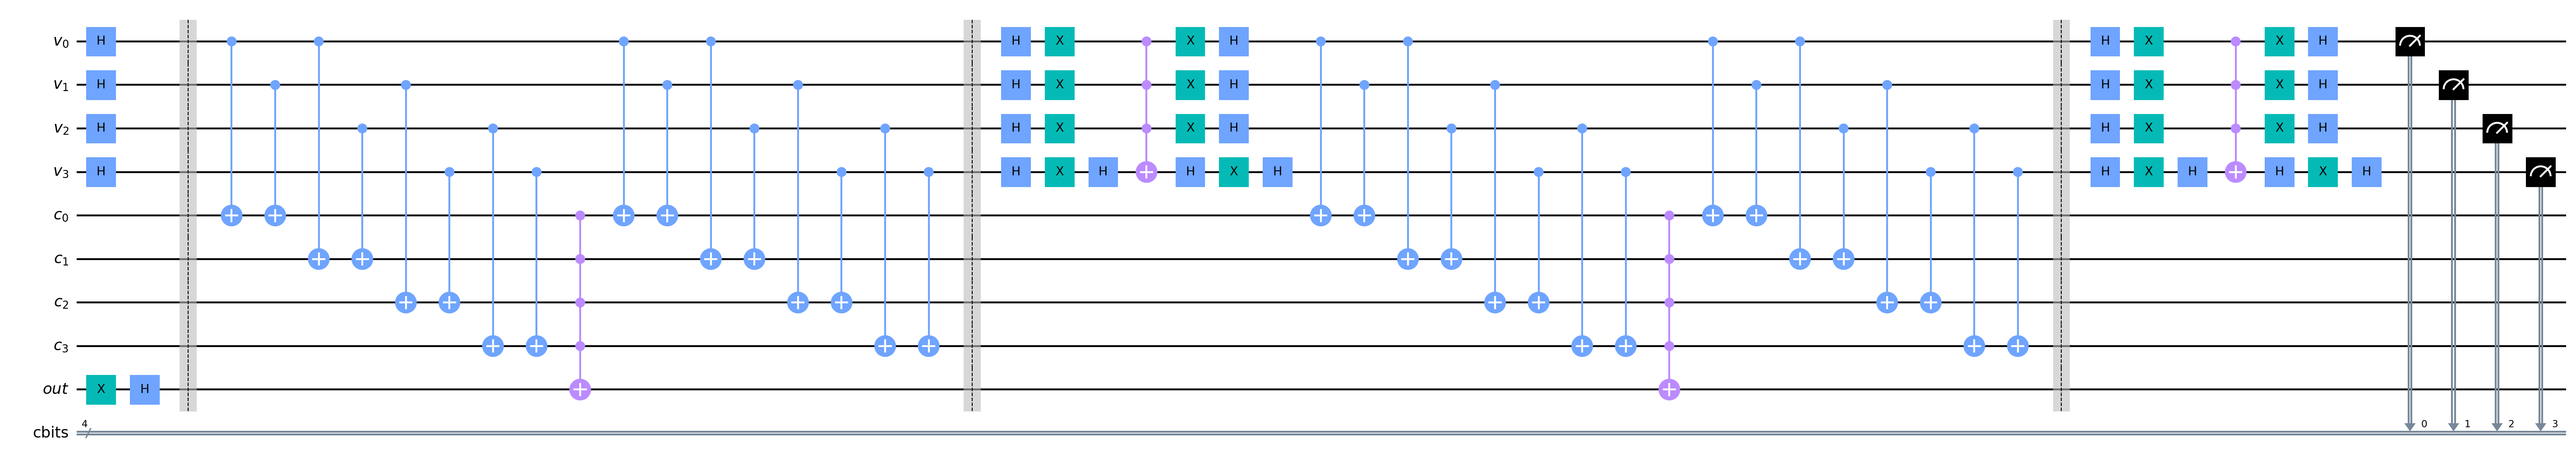
\includegraphics[width=1\linewidth]{../Code/3-Fig_Sudoku_2x2.png}
	\caption{Circuito completo para la resolución con Grover del sudoku 2x2. Código en 
	Grover's\_algoritm$\backslash$Code$\backslash$sudoku\_2x2.py}
	\label{Fig_Imple_Sudoku_2x2}
	\end{figure}
	
	\begin{figure}[H]
	\centering 
	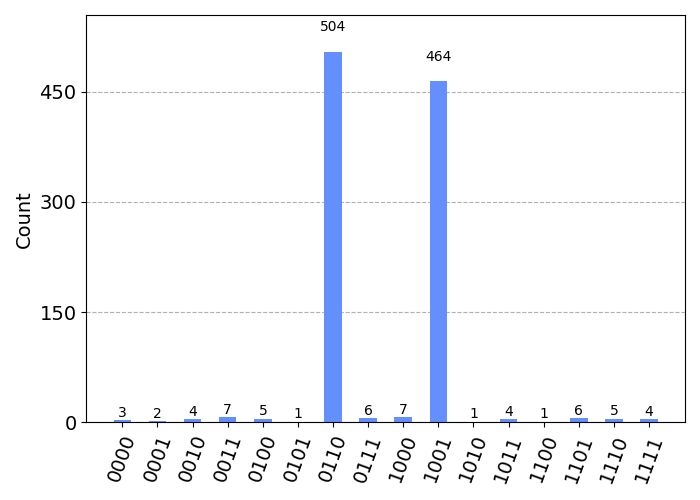
\includegraphics[width=0.6\linewidth]{../Code/3-Fig_Sudoku_2x2_Histogram.png}
	\caption{Resultado de la simulación del circuito de la Fig. \ref{Fig_Imple_Sudoku_2x2}.}
	\label{Fig_Imple_Oracle_Sudoku_2x2_Histogram}
	\end{figure}

	\begin{mybox}{Nota}
	El código que generó las simulación de las Figs. \ref{Fig_Imple_Sudoku_2x2} y 
	\ref{Fig_Imple_Oracle_Sudoku_2x2_Histogram} puede encontrarse en el script	
	\textbf{3-Sudoku\_2x2.py} en la carpeta \textbf{Grover's\_algoritm$\backslash$Code}.
	\end{mybox}


\subsubsection{Permutaciones de P números.}

En esta sección vamos a ver como construir un oráculo que nos dé todas las permutaciones posibles de $P$ números $v_0v_1 \dots v_{p-1}$ (con $P$ siendo una potencia de 2). Para construir este oráculo necesitamos 4 registro de qubits:
\begin{itemize}
	\item \textit{var\_reg}: Es el registro donde se almacenan los número que queremos que verifiquen las condiciones. Debe de tener $P*p$ qubits, donde $p$ es el número de bis necesario para representar $P$ en binario. Por ejemplo, para $P=4$ necesitamos 8 qubits.
	
	\item \textit{ancilla\_reg}: Este registro lo usamos para compara qubit a qubit (bit a bit) los números codificados en el registro anterior. Debe de tener $p$ qubits.
	
	\item \textit{ancilla\_reg\_2}: Este registro tendrá tantos qubits como condiciones deben de verificarse. En cada qubit de este registro se almacenara el resultado de cada una de las condiciones (0 si no se cumple, 1 si se cumple). Para $P$ número tenemos $(P-1)!$ condiciones. Por ejemplo, para $P=4$ tenemos:
	$$
	v_0 \neq v_1, \quad v_0 \neq v_2, \quad v_0 \neq v_3, \quad v_1 \neq v_2, \quad v_1 \neq v_3, \quad v_2 \neq v_3
	$$
	
	\item \textit{ancilla\_out\_qubit}: Un registro con un solo qubit. Este qubit está en el estado $|-\rangle$ y sobre el se aplicará una puerta $X$ si todos los qubits del registro \textit{ancilla\_reg\_2} están en el estado $|1 \rangle$ (es decir, si se cumplen todas las condiciones).
\end{itemize}

En las Figs. \ref{Fig_permitaciones_oracle_1.png} y \ref{Fig_permitaciones_oracle_2.png} podemos ver la primera parte del oráculo para el caso de $P=4$.  Podemos ver que está dividido en 7 bloques: un bloque por cada condición más un último bloque con un MCT que se aplica tomando como controles todos los qubit del registro {ancilla\_reg\_2} y que tiene como objetivo el qubit \textit{ancilla\_out\_qubit}. 

Cada uno de los 6 bloques realiza una comparación bit a bit de dos números (compara el primer bit con el primero, el segundo con el segundo,...). Cada comparación se realiza usando 2 CNOT. Una de ellas controlada por uno de los bits y la otra por el otro. Las CNOTs tiene como qubit objetivo un qubit del registro \textit{ancilla\_reg} ($c_0, c_1, \dots$). De esta forma, si los bis son diferentes el estado del qubit del registro \textit{ancilla\_reg} pasa a ser $|1\rangle$. Para nuestro caso de $P=4$, estas comparaciones las realizan las primeras 4 CNOTs de cada bloque.

Dos números son diferentes si al menos uno de sus bits es diferente, es decir, si tenemos al menos un $|1\rangle$ en el registro \textit{ancilla\_reg} después de las comparaciones de parágrafo anterior. El siguiente tramo de los bloques actúa sobre los qubits del registro \textit{ancilla\_reg} y un qubit del registro \textit{ancilla\_reg\_2} ($c\_out_0, c\_out_1, \dots$). El objetivo el mismo es poner el qubit del registro \textit{ancilla\_reg\_2} en el estado $|1\rangle$ si tenemos al menos un $1$ en el registro \textit{ancilla\_reg}. Esto lo hacemos en tres pastes:
\begin{enumerate}
	\item Aplicamos sobre el qubit del registro \textit{ancilla\_reg\_2} una CNOT por cada qubit del registro \textit{ancilla\_reg}. De esta forma, estamos cambiando el estado del qubit objetivo si tenemos un número impar de 1's en el registro \textit{ancilla\_reg}.
	
	\item Aplicamos un puerta $X$ sobre uno de los qubits de \textit{ancilla\_reg}. Volvemos a aplicar las CNOT y tras ellas volvemos a aplicar la puerta $X$. De esta forma, estamos cambiando el estado del qubit objetivo si tenemos un número par de 1's en el registro \textit{ancilla\_reg} o ningún 1 (si tenemos todo 0's) 
	
	\item Aplicamos puertas $X$ sobre todos los qubis del registro \textit{ancilla\_reg}, aplicamos una MCT y aplicamos otra vez puertas $X$ en todos los qubit de \textit{ancilla\_reg}. De esta forma, corregimos el hecho de haber cambiado el estado del qubit objetivo en el caso de haber tenido un estado con todo ceros en el registro \textit{ancilla\_reg}.
	
\end{enumerate}

La última parte de los bloques es volver a aplicar las CNOT de comparación del circuito para limpiar los qubits del registro \textit{ancilla\_reg}.

La segunda parte del oráculo consistiría en repetir los 6 bloques (en realidad, los $(P-1)!$ bloques) de las condiciones para volver a poner a cero los qubits del registro {ancilla\_reg\_2}.

	\begin{figure}[H]
	\centering 
	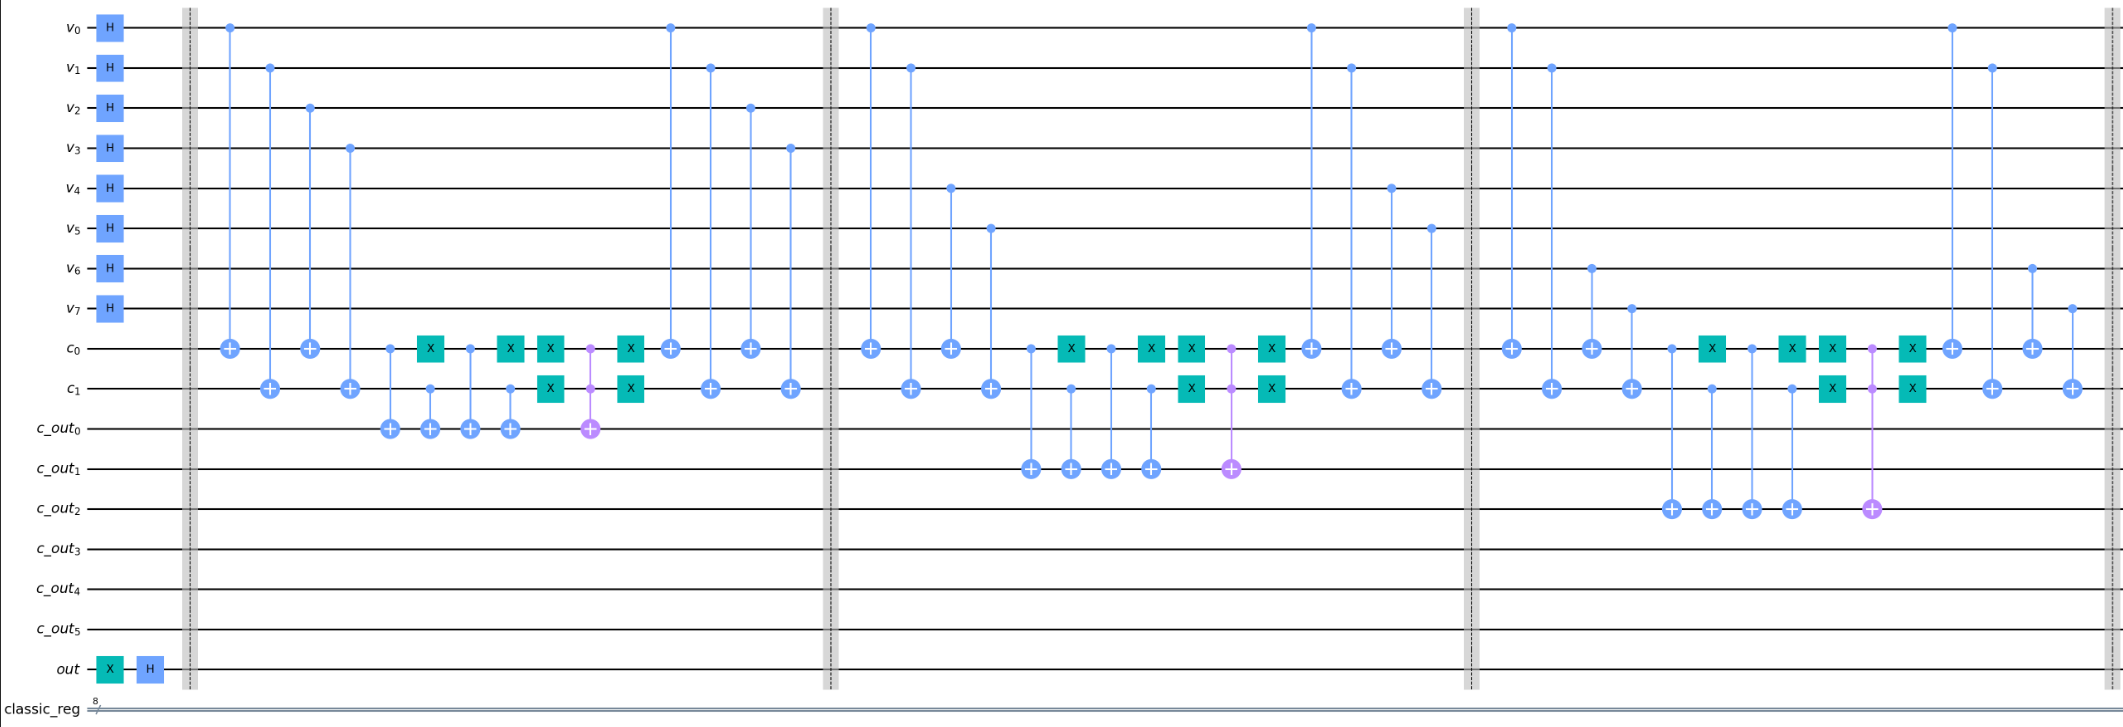
\includegraphics[width=1\linewidth]{Figuras/Fig_permitaciones_oracle_1.png}
	\caption{Oráculo para calcular las permutaciones, parte uno primer tramo.}
	\label{Fig_permitaciones_oracle_1.png}
	\end{figure}

	\begin{figure}[H]
	\centering 
	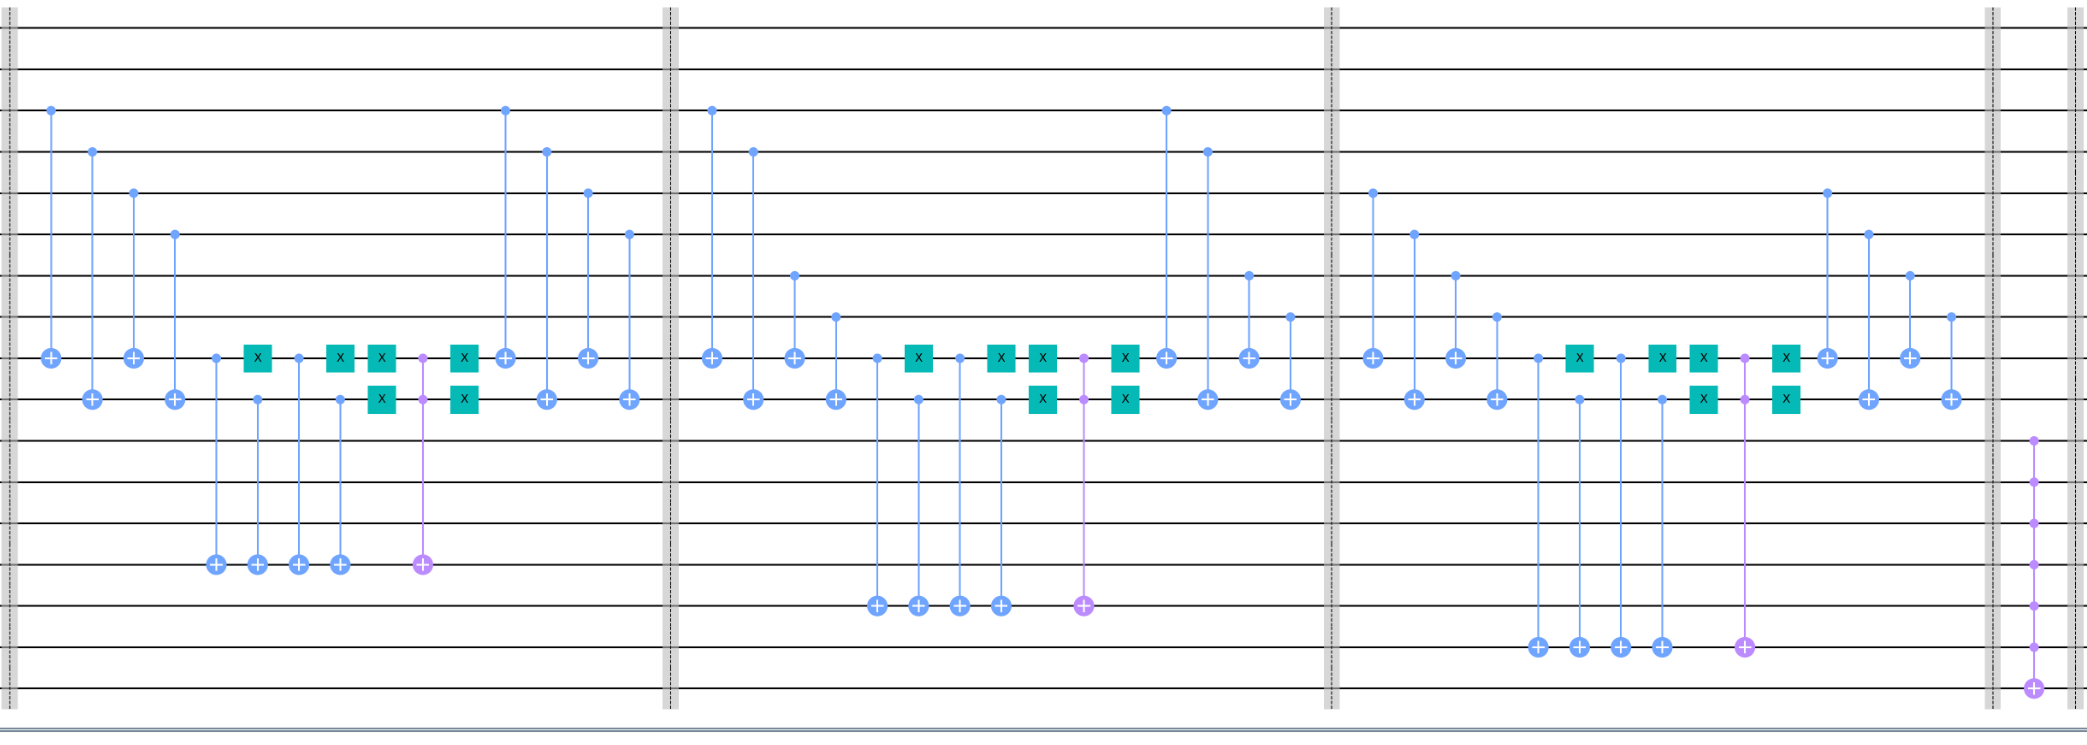
\includegraphics[width=1\linewidth]{Figuras/Fig_permitaciones_oracle_2.png}
	\caption{Oráculo para calcular las permutaciones, parte uno segundo tramo.}
	\label{Fig_permitaciones_oracle_2.png}
	\end{figure}

\begin{mybox_red}{Nota Importante!!}
Puede verse una implementación más general y avanzada del caso de las permutaciones situado en la carpeta \textbf{Grover's\_algoritm$\backslash$Code.} (en mismo nivel que la carpeta Theory). En esta implementación se usa la idea de buscar números diferentes para calcular las permutaciones de $P$ números. Esta implementación es la ``joya de la corona'' de la explicación que se está dando sobre el algoritmo de Grover.
\end{mybox_red}


%\section{Invertir una función}

%\textcolor{red}{No se si haré algo en esta sección}

%An alternate view of Grover’s algorithm can be ”inverting a function” instead of ”searching a database”. Given a function y = f(x) that can be evaluated on a quantum computer, Grover’s algorithm can calculate x. 
















% Bibliografía

%\newpage
\nocite{*}
\bibliographystyle{ieeetr}
\bibliography{Grover-Algorithm_Bibliografia}

\end{document}